\chapter{RadGrad System}
\label{radgrad-system}

I believe that the best way to address current ICS student issues is through an online system that combines degree planning, social networking, and gamification. The specific features of the system evolved over time through a process conducted in Fall 2015-Spring 2016 by Philip Johnson. This process incorporated feedback from the four major RadGrad user groups: students, faculty, academic program advisers, and alumni/local high tech community members. Spring 2015 students in Software Engineering II became directly involved in the design process by creating their own paper and HTML mockups and by doing user tests and analyses on their suggested systems. Faculty members and academic program advisers provided feedback through a RadGrad advisory board and through advising sessions. Alumni and local high tech community members became involved through RadGrad talks at local tech meetups. 

Development of the current RadGrad system began in September 2016. We first created mockups based off the system requirements presented in the System Design section. We then decided on a few key design patterns to follow (i.e. color schemes, layouts, general site organization, etc.). Over the next few months, we continued to change and narrow down our design, until we were able to deploy a working beta version for students, advisors, and alumni. We were then able to test the system with real users, and use the feedback to further improve upon the system. In this chapter, I present the current state of the RadGrad system as of June 2017.
\vspace{5mm}
\section{Development}
\subsection{Frameworks and Environments}

RadGrad was built using the Meteor JavaScript web framework. Meteor is integrated with MongoDB and uses the Distributed Data Protocol and publish-subscribe pattern to create real time, responsive code that automatically updates data changes to the client. On the client side, RadGrad uses jQuery and Semantic UI to design and create the user interface. Due to excellent Meteor integration, RadGrad was developed using IntelliJ IDEA. In an effort to create clean and uniform code, RadGrad uses ESLint to confrom to the AirBnB Javascript Style Guide. 

\subsection{Project Management}

We developed RadGrad using GitHub issues and GitHub projects. Development tasks are created as a GitHub issue, and each issue has an assigned developer and and assigned branch. Each issue also resides in a GitHub project, which groups issues together to mark larger milestones. We track issues using a ``Backlog", ``In Progress", and ``Done" column. The RadGrad developers typically communicate through Slack and in person meetings twice a week. 

\section{RadGrad Users}

There are currently five different types of RadGrad users: administrators, advisors, faculty, mentors, and students. Administrators can be RadGrad team members, or UHM academic advisors or faculty that request access. Advisors are UHM academic advisors for ICS students. Faculty members include all professors in the ICS department. Mentors include any ICS alumni that desire to give back to the ICS community. Students include all currently enrolled ICS undergraduate students. 

\section{Student Components}

The three main RadGrad themes (degree planner, social networking, and gamification) are manifested through several different components throughout the system. In this section, I describe all of these components from the student point of view. Refer to Appendix \ref{other-radgrad-components} to view these components from the point of view of other user types.

\subsection{Degree Planning}

There are degree planner components on the degree planner page (Figure \ref{degree-planner-page}), explorer pages, the student home page (Figure \ref{student-home-page}). In the following section, I will describe the degree planner components in further detail. 

\subsubsection{Degree Planner}
\begin{figure}[htbp!]
\centering
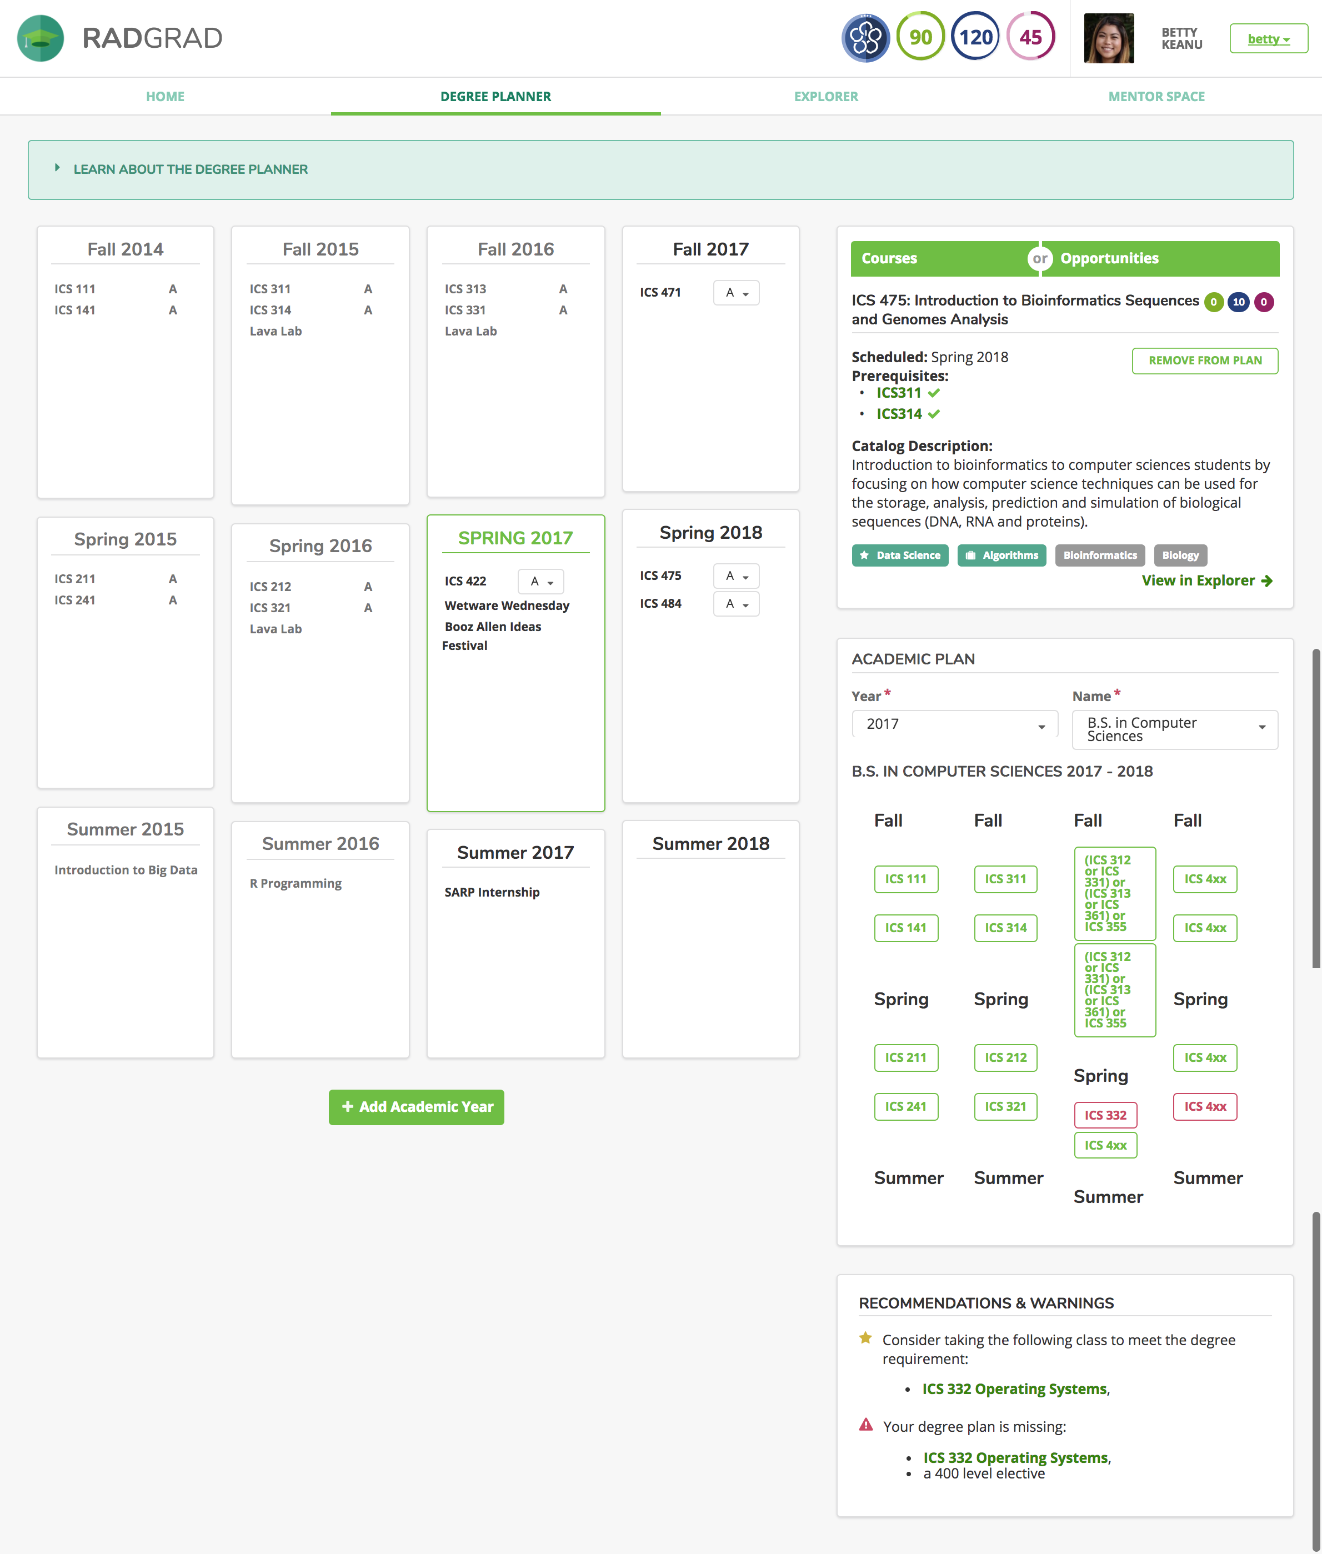
\includegraphics[width=1.0\textwidth]{degree-planner}
\caption{Degree planner page.}
\label{degree-planner-page}
\end{figure}

\begin{figure}[htbp!]
\centering
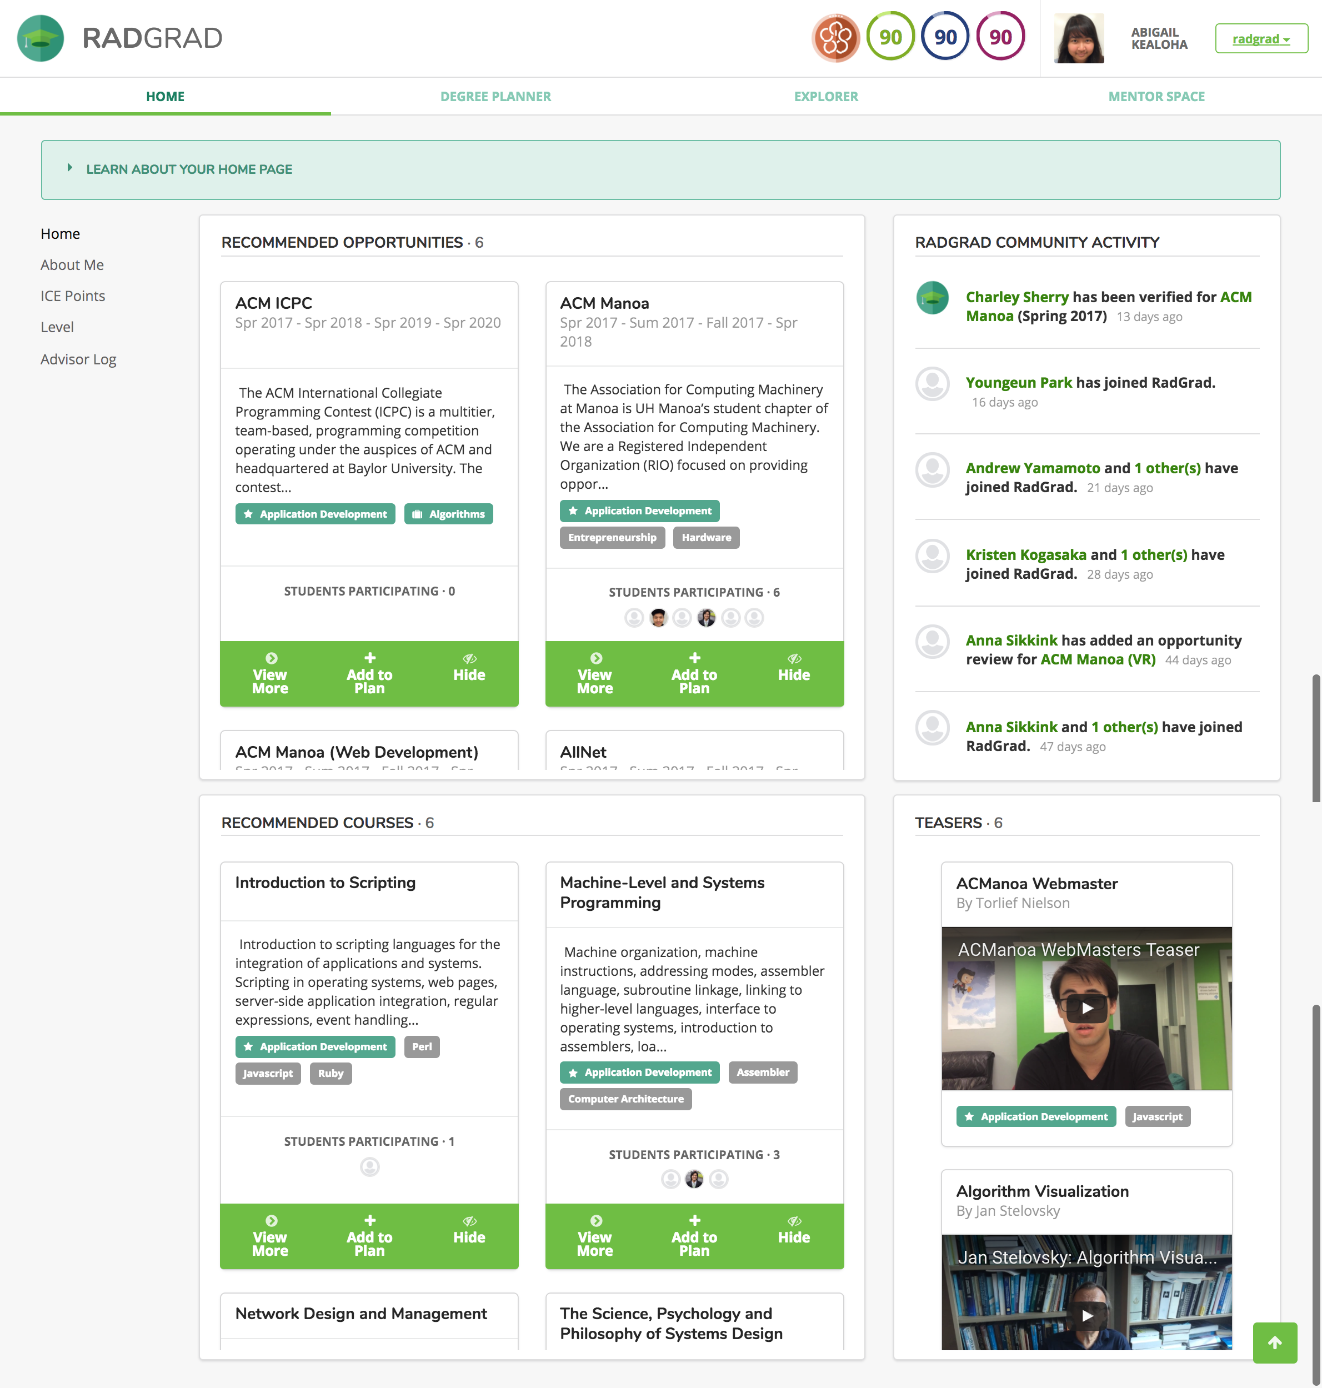
\includegraphics[width=1.0\textwidth]{student-home}
\caption{Student home page with teasers, feed, and recommended courses and opportunities.}
\label{student-home-page}
\end{figure}

\begin{figure}[htbp!]
\centering
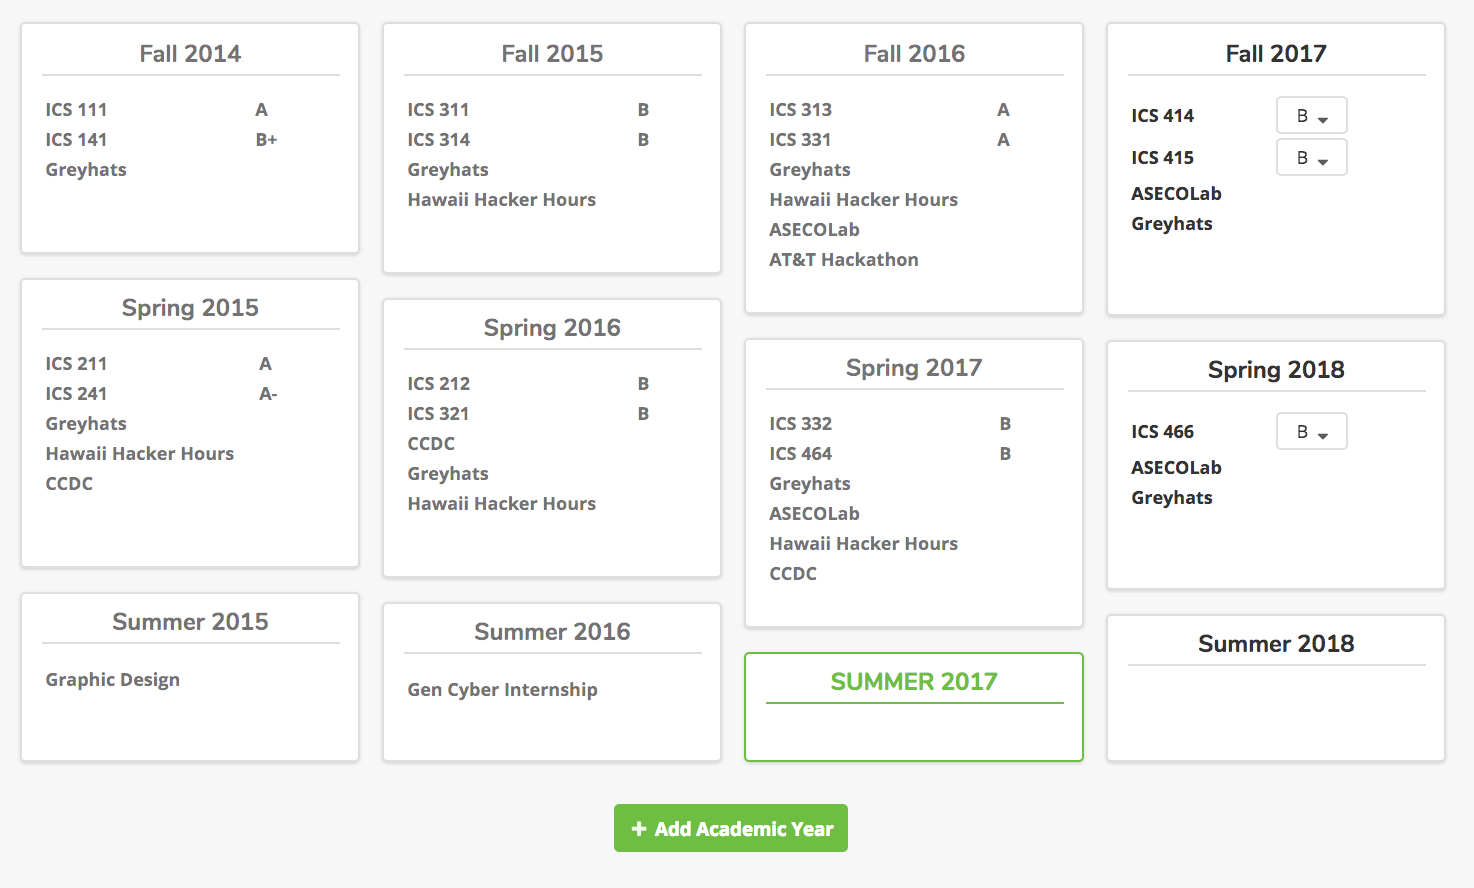
\includegraphics[width=1.0\textwidth]{dp-dp}
\caption{Close up of degree plan on the degree planner page.}
\label{degree-planner}
\end{figure}

The student degree planner was created to help students increase their extracurricular engagement in a way that makes sense for their specific path and fits into their time constraints ( Figure ~\ref{degree-planner}, Figure ~\ref{degree-planner-page}). The student degree planner is the main place that students will go to view and make changes to their entire degree plan. Students can view up to four academic years at a time, but they can view additional past or future years by clicking on the green arrows at the bottom. Semesters that are in the past are greyed out and cannot be changed by the student. Any present or future semesters can be changed by dragging and dropping courses or opportunities into that semester pane. The grades for a course can be changed with the drop down menus. 

\begin{figure}[htbp!]
\centering
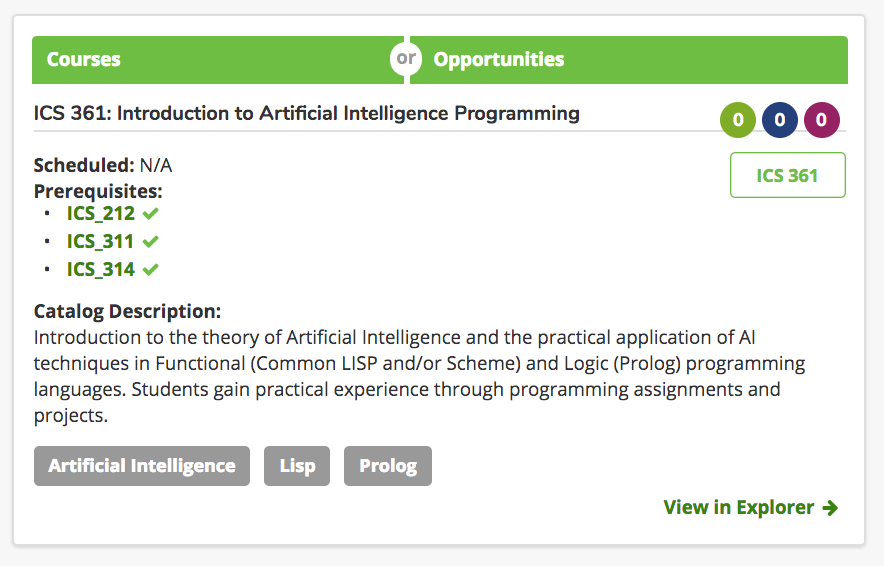
\includegraphics[width=1.0\textwidth]{dp-viewer}
\caption{Close up of the inspector on the degree planner page.}
\label{inspector}
\end{figure}

This page also includes an inspector pane on the top right hand corner, which the student can use to view brief details about a course or opportunity while planning their degree (Figure ~\ref{degree-planner-page}, Figure ~\ref{inspector}). The in-depth course and opportunity explorer pages can be accessed through the inspector, but the short descriptions in the inspector allows for quick and convenient assistance within the same view as the degree planner itself. The student can choose a course or opportunity to inspect by either choosing from the green dropdown menu at the top of the inspector, or by clicking on the course or opportunity name within the plan. 

\begin{figure}[htbp!]
\centering
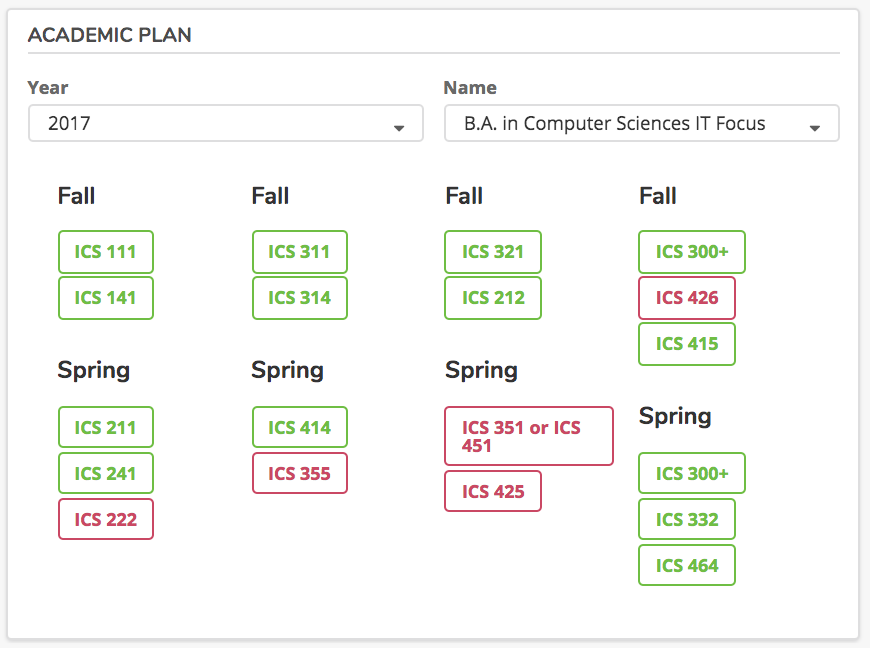
\includegraphics[width=1.0\textwidth]{dp-academicplan}
\caption{Close up of academic plans on the degree planner page.}
\label{academic-plans}
\end{figure}
Below the inspector is the academic plan pane (Figure ~\ref{academic-plans}, Figure ~\ref{degree-planner-page}). In this pane, students can select a year and an academic plan name (i.e. B.S. in Computer Science Security Science) to indicate the degree plan that the would like to follow. The pane then displays the required courses for this plan, organized into the recommended semesters, and color coded (green for classes in the student's plan, and red for classes not in the student's plan). Students can use this display to easily drag their missing courses onto their plan.

\begin{table}[htbp!]
\centering
\begin{tabular}{  |p{4cm}|p{12cm}| } 
\hline
 \multicolumn{2}{|c|}{Potential Areas the Degree Planner Could Improve}\\
  \hline
 \textbf{TechHui Complaints} & \textbf{Reasoning} \\ 
  \hline
ICS department should offer classes more frequently & Advisors will be able to gather data about which future classes students are interested in, and advisors will be able to schedule these classes with the students' needs in mind. \\
\hline
 \textbf{Survey Questions} & \textbf{Reasoning} \\ 
  \hline
  How many extracurriculars have you participated in? & The RadGrad degree planner encourages students to add both courses and opportunities to their schedules.\\
  \hline
  How well prepared do you feel to find a job after graduation? & The RadGrad degree planner encourages students to plan ahead, be more in control of their degree plans, and to include both courses and opportunities, which can make students more confident and competitive when finding jobs.\\
  \hline
\end{tabular} 
\caption{Potential Areas the Degree Planner Could Improve}
\end{table}

\subsubsection{Recommendations and Warnings}

\begin{figure}[htbp!]
\centering
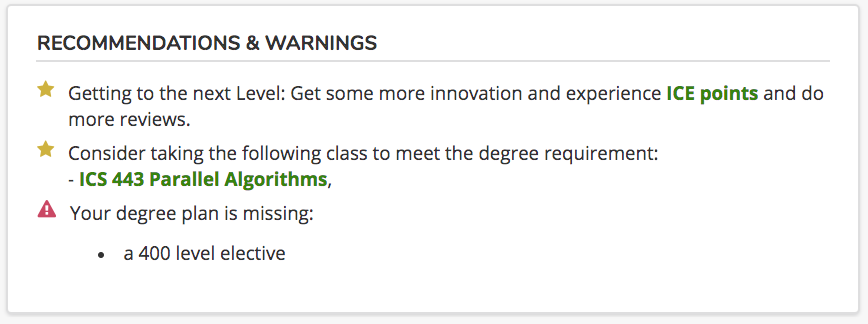
\includegraphics[width=1.0\textwidth]{dp-rw}
\caption{Close up of recommendations and warnings on the degree planner page.}
\label{recommendations-warnings}
\end{figure}

The student degree planner automatically generates warnings and recommendations on the bottom right hand corner (Figure ~\ref{recommendations-warnings}, Figure ~\ref{degree-planner-page}). These warnings and recommendations change as a student's degree plan changes. Each time a student adds, moves, or removes a course or opportunity through the degree planner, explorer, or student home page, the warnings and recommendations will regenerate. All possible warnings and recommendations as of June 2017 are listed in Table ~\ref{table:warnings-recommendations}. These recommendations and warnings were created to help make the process of integrating courses and opportunities into a chosen time frame easier.

\begin{figure}[htbp!]
\centering
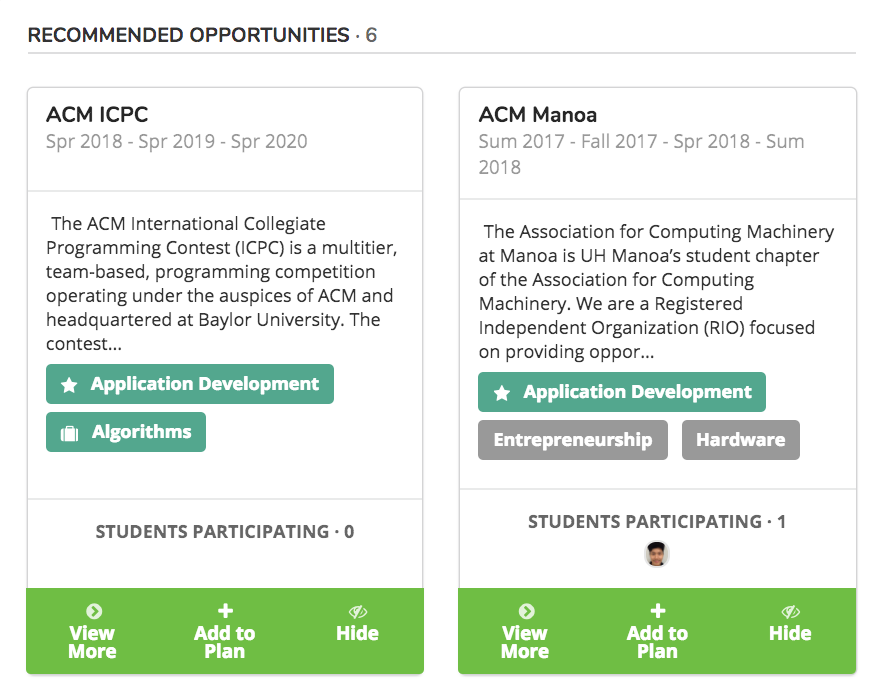
\includegraphics[width=1.0\textwidth]{home-recommend}
\caption{Close up of recommendations on the student home page.}
\label{home-recommend}
\end{figure}

On the student home page, students can see details about recommended courses and opportunities as soon as they log in (Figure ~\ref{home-recommend}, Figure ~\ref{student-home-page}). These are chosen based off the student's chosen interests and career goal related interests. If a student is interested in a particular course or opportunity, they can choose to view more in the explorer, add it to their plan, or leave it there to decide what to do with later. If a student knows they are not interested in a certain course or opportunity, they can choose to hide it by clicking the "hide" button. If the student later changes their mind, they can view and unhide the course or opportunity by clicking ``Hidden Opportunities." These home page recommendations were created to help make the process of choosing and integrating interesting courses and opportunities easier and less overwhelming.


\begin{table}[htbp!]
\centering
\begin{tabular}{  |p{8cm}|p{8cm}| } 
  \hline
 \textbf{Warnings} & \textbf{Recommendations} \\ 
  \hline
A prerequisite course is missing & Course recommended based upon interests\\
\hline
Semester appears overloaded (more than 3 ICS courses) & Opportunity recommended based upon interests\\
\hline
A required course is missing & Recommendation for ICS innovation points \\
\hline
Course is not offered in chosen semester (future implementation) & Recommendation for ICS competency points \\
\hline
& Recommendation for ICS experience points\\
\hline
& Move towards achieving the next level \\
\hline
& See your ICS advisor to upload STAR data\\
 \hline
\end{tabular}
\caption{Automatically generated warnings and recommendations as of May 2017}
\label{table:warnings-recommendations}
\end{table}

\begin{table}[htbp!]
\centering
\begin{tabular}{  |p{4cm}|p{12cm}| } 
\hline
 \multicolumn{2}{|c|}{Potential Areas Warnings and Recommendations Could Improve}\\
\hline
 \textbf{Survey Questions} & \textbf{Reasoning} \\ 
  \hline
  How many extracurriculars have you participated in? & Recommendations encourage students to add opportunities to their schedules that match their individual interests, which could cause students to find and participate in more extracurriculars.\\
  \hline
  How well prepared do you feel to find a job after graduation? & Recommendations and warnings help students to take all the required courses, and also help students to add more courses and opportunities of interest to their degree plans, which can make students feel more confident and in control of how they prepare for life after graduation. \\
  \hline
\end{tabular}
 \caption{Potential Areas Warnings and Recommendations Could Improve}
\end{table}

\subsubsection{Career Goal, Course, Desired Degree and Opportunity Explorers}

Students can access the career goal, course, desired degree, and opportunity explorers to help them plan their degree.  These explorers can be accessed through the ``Explorer" top menu on the student home page. The specific explorer can be chosen using the dropdown menu on the left side. These explorers were created to help make the process of combining career goals, courses, degrees, and opportunities together into a cohesive degree plan faster and easier. Students can go to one place to find all of the information they need to piece their plan together, rather than having to depend on a number of external sources.

\begin{figure}[htbp!]
\centering
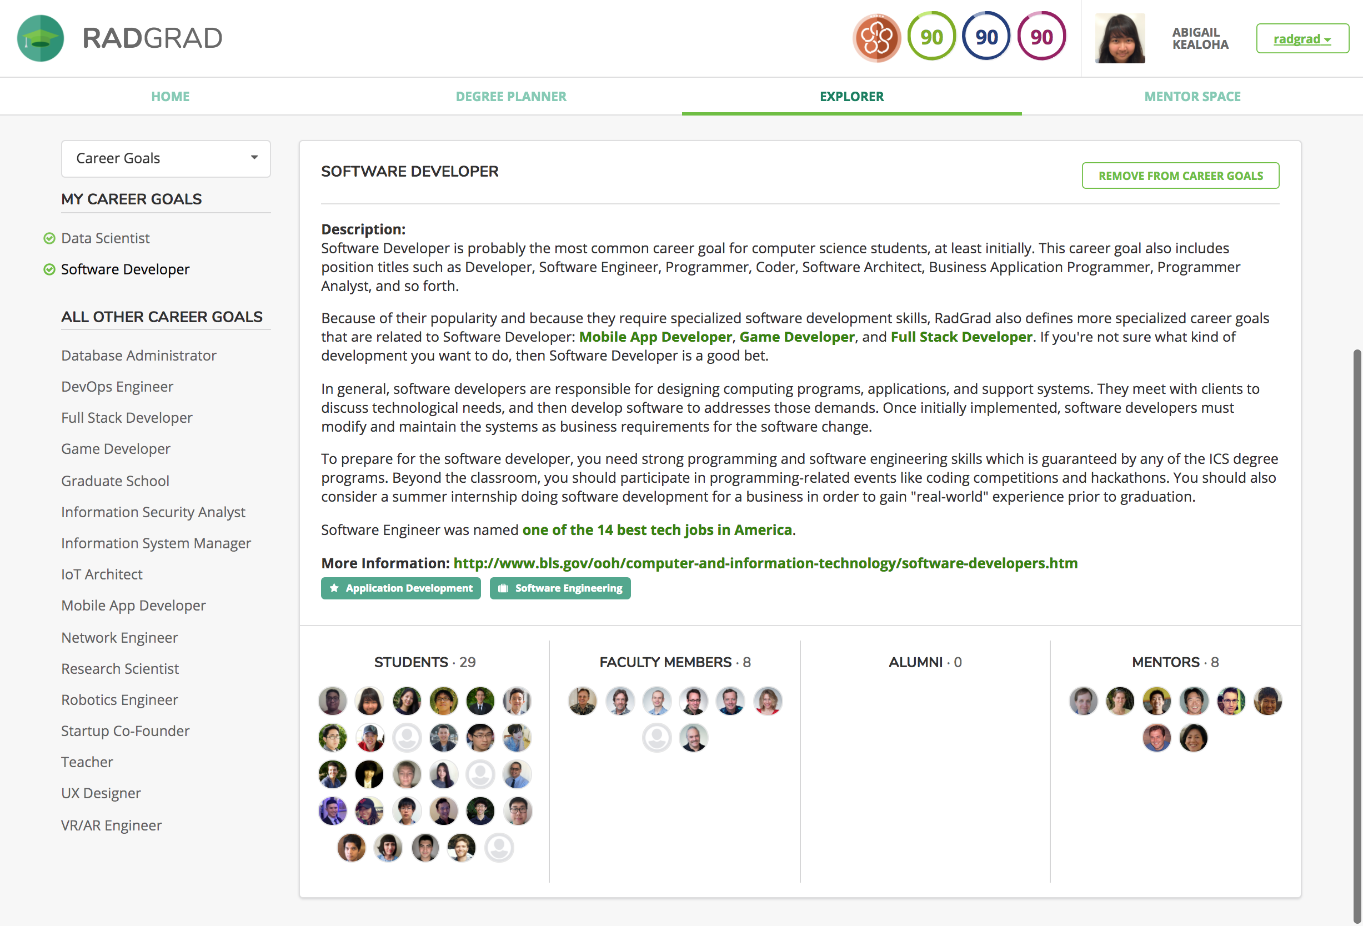
\includegraphics[width=1.0\textwidth]{careergoal-explorer}
\caption{Career goal explorer page.}
\label{career-goal-explorer}
\end{figure}

The career goal explorer lists all RadGrad career goals on the left side (Figure ~\ref{career-goal-explorer}). These career goals are arranged by ``My Career Goals" (career goals that the user has added) and ``All other career goals" (career goals that the user has not added). The user can click on a career goal to view details about that career goal. These details include a description of the career goal, related interests, related courses and/or opportunities, a link for more information, interested students, interested faculty, interested alumni, and interested mentors. On this page, the user can also add or remove the career goal by clicking on the green button at the top right corner.  

\begin{figure}[htbp!]
\centering
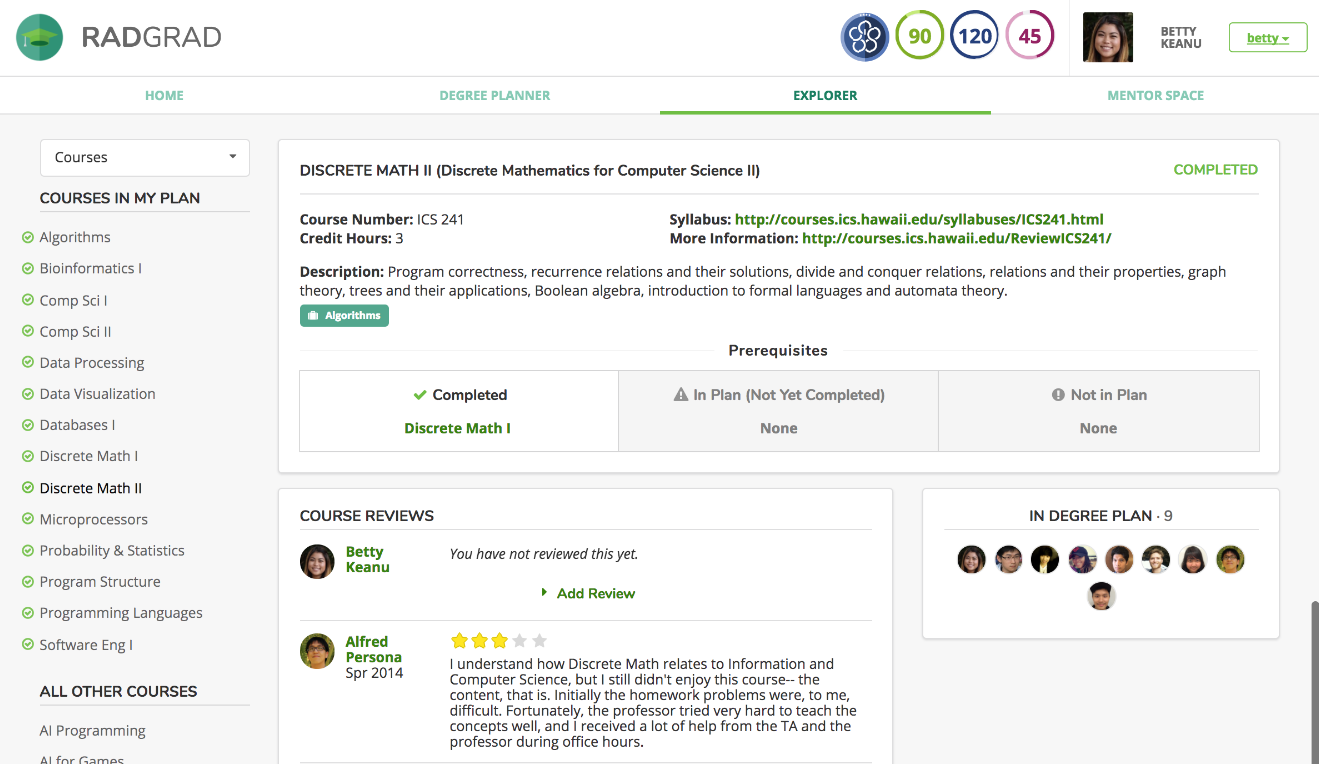
\includegraphics[width=1.0\textwidth]{course-explorer}
\caption{Course explorer page.}
\label{course-explorer}
\end{figure}

The course explorer lists all RadGrad courses on the left side (Figure ~\ref{course-explorer}). These courses are arranged by ``Courses in my Plan" (all past, present or future courses in the student's degree plan) and ``All Other Courses" (courses not in the user's degree plan). The user can click on a course to view details about that course. These details include course number, a link to the syllabus, credit hours, a description of the course, prerequisites, organized into three categories (completed, in plan but not yet completed, and not in plan), and a list of students with this course in their degree plan. On this page, users can also view course reviews from other students and add or edit their own course review. The user can add or remove this course from their degree plan by clicking on the green button at the top right corner. If the user has already taken and passed the course, they cannot add it again.

\begin{figure}[htbp!]
\centering
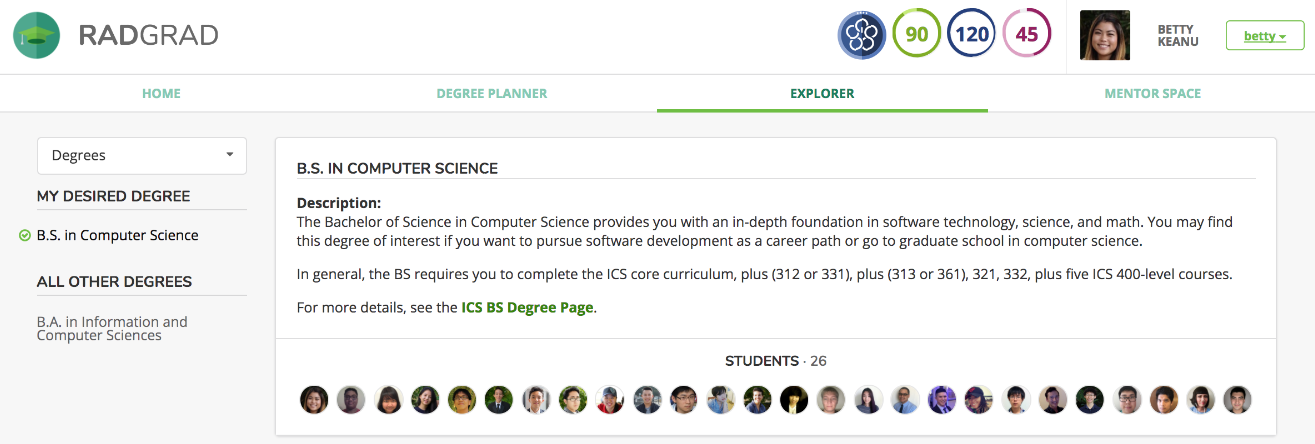
\includegraphics[width=1.0\textwidth]{degree-explorer}
\caption{Degree explorer page.}
\label{degree-explorer}
\end{figure}

The degree explorer lists all possible ICS degrees on the left side (Figure ~\ref{degree-explorer}). These degrees are arranged by ``My Desired Degree" (the student can only have one desired degree at a time), and ``All Other Degrees" (degrees not currently chosen as the user's desired degree). The user can click on a degree to view details about that degree. These details include a description, where to go for more information, and a list of students who have this degree listed as their current desired degree. On this page, users can set a new degree goal by clicking on the green button at the top right corner.

\begin{figure}[htbp!]
\centering
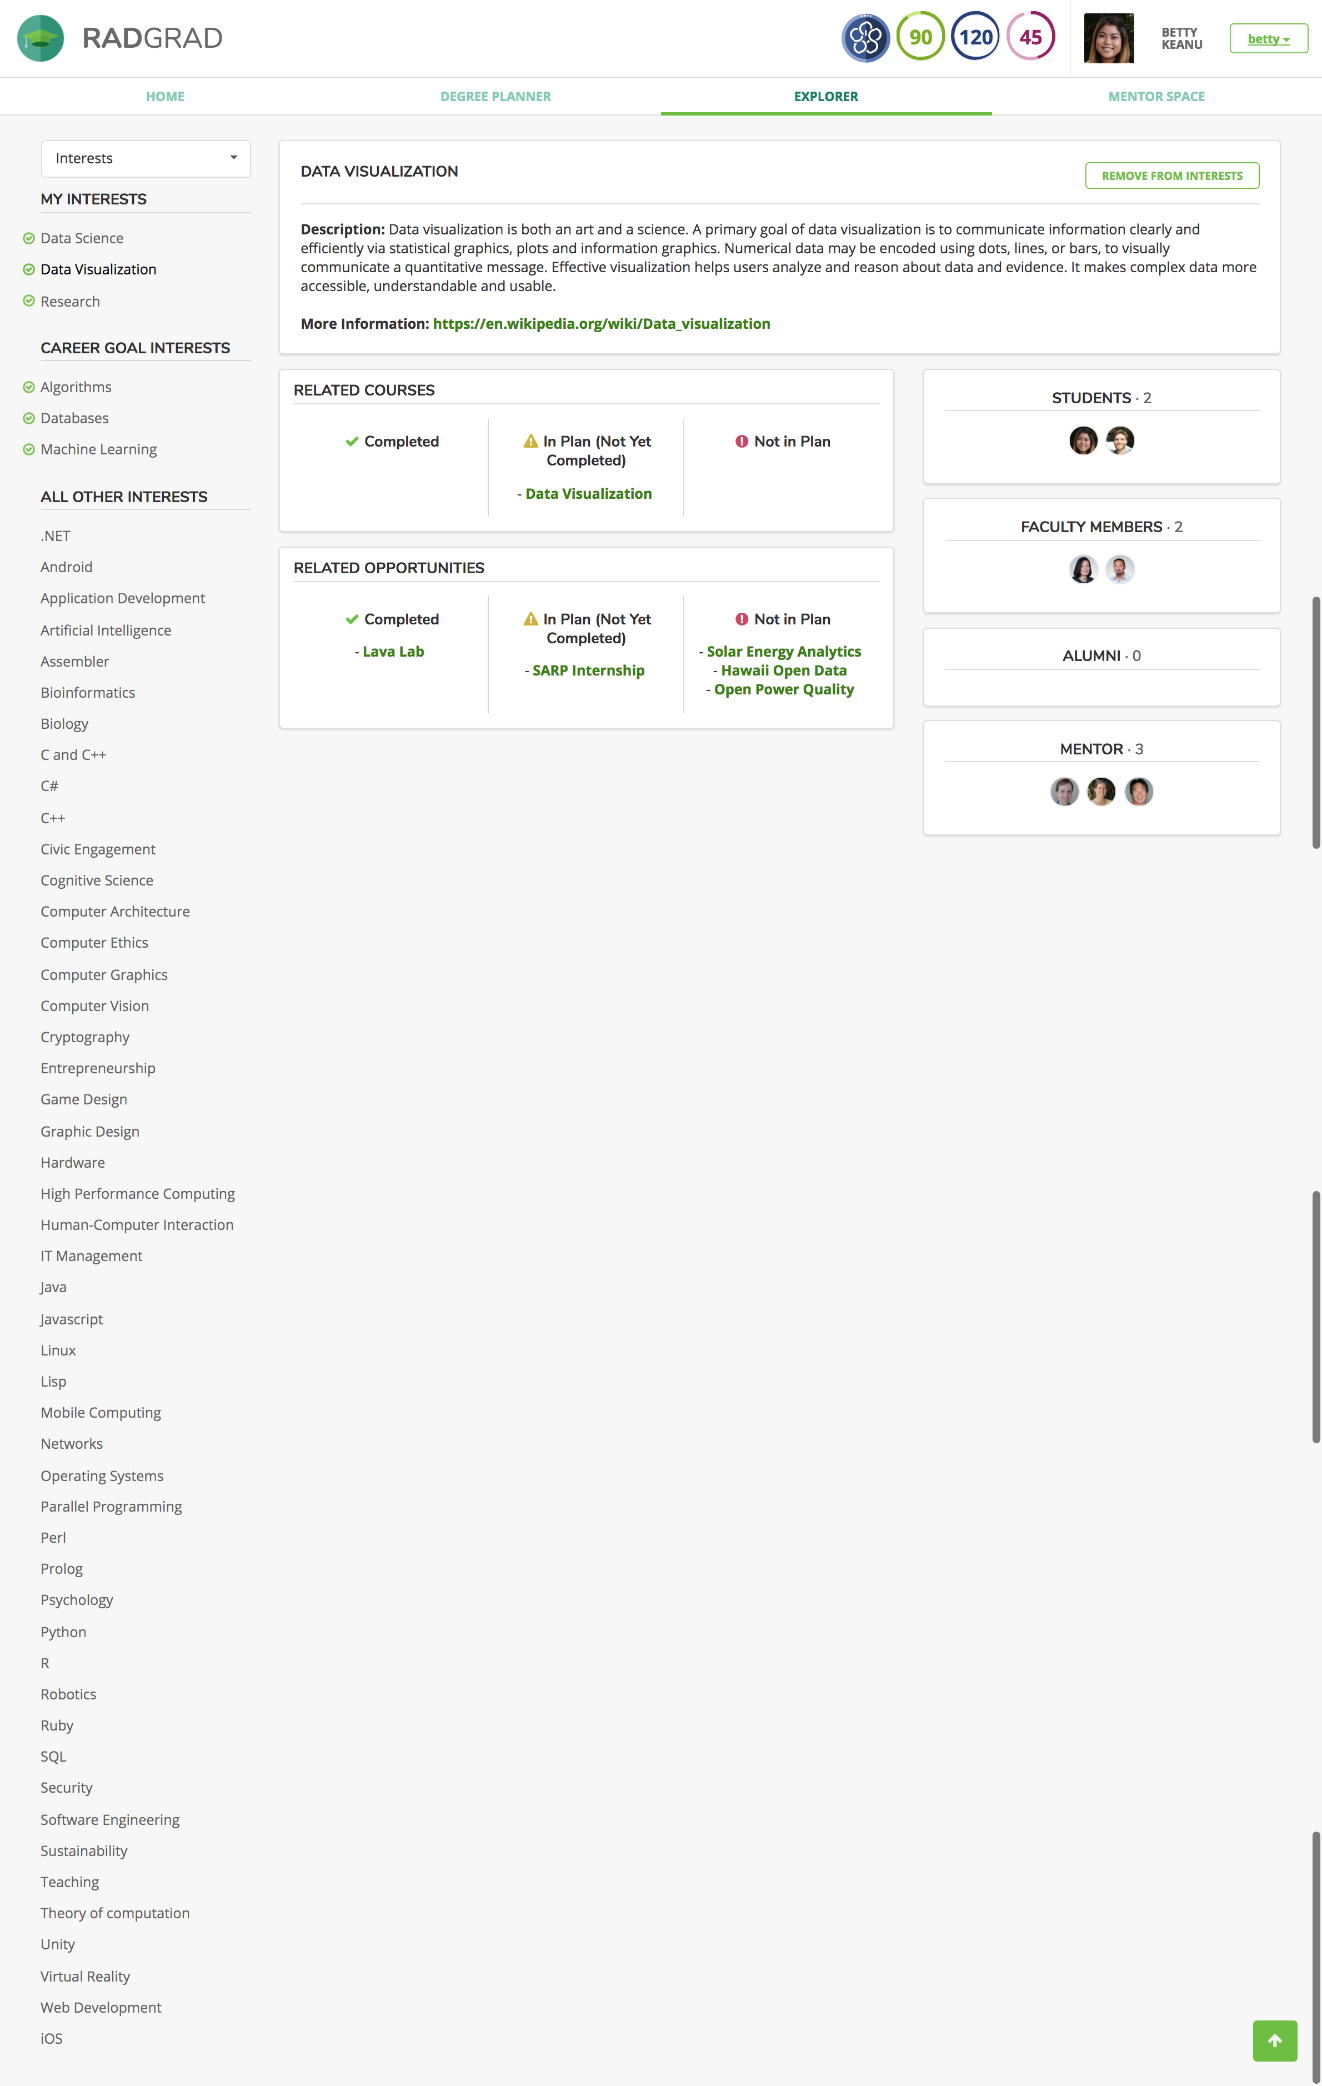
\includegraphics[width=1.0\textwidth]{interest-explorer}
\caption{Interest explorer page.}
\label{interest-explorer}
\end{figure}

The interest explorer lists all possible RadGrad interests on the left side (Figure ~\ref{interest-explorer}). These interests are arranged by ``My Interests" (interests that the user has added), ``Career Goal Interests" (interests that have automatically been added due to their association with one or more of the user's chosen career goals), and ``All Other Interests" (interests that the user has not added and are not related to any of the user's career goals). The user can click on an interest to view details about that interest. These details include a description of the interest, related courses and related opportunities, both organized into three categories (completed, in plan but not yet completed, and not in plan), and students, faculty, alumni, and mentors who have added this interest. On this page, users can also add or remove the interest by clicking on the green button at the top right corner.

\begin{figure}[htbp!]
\centering
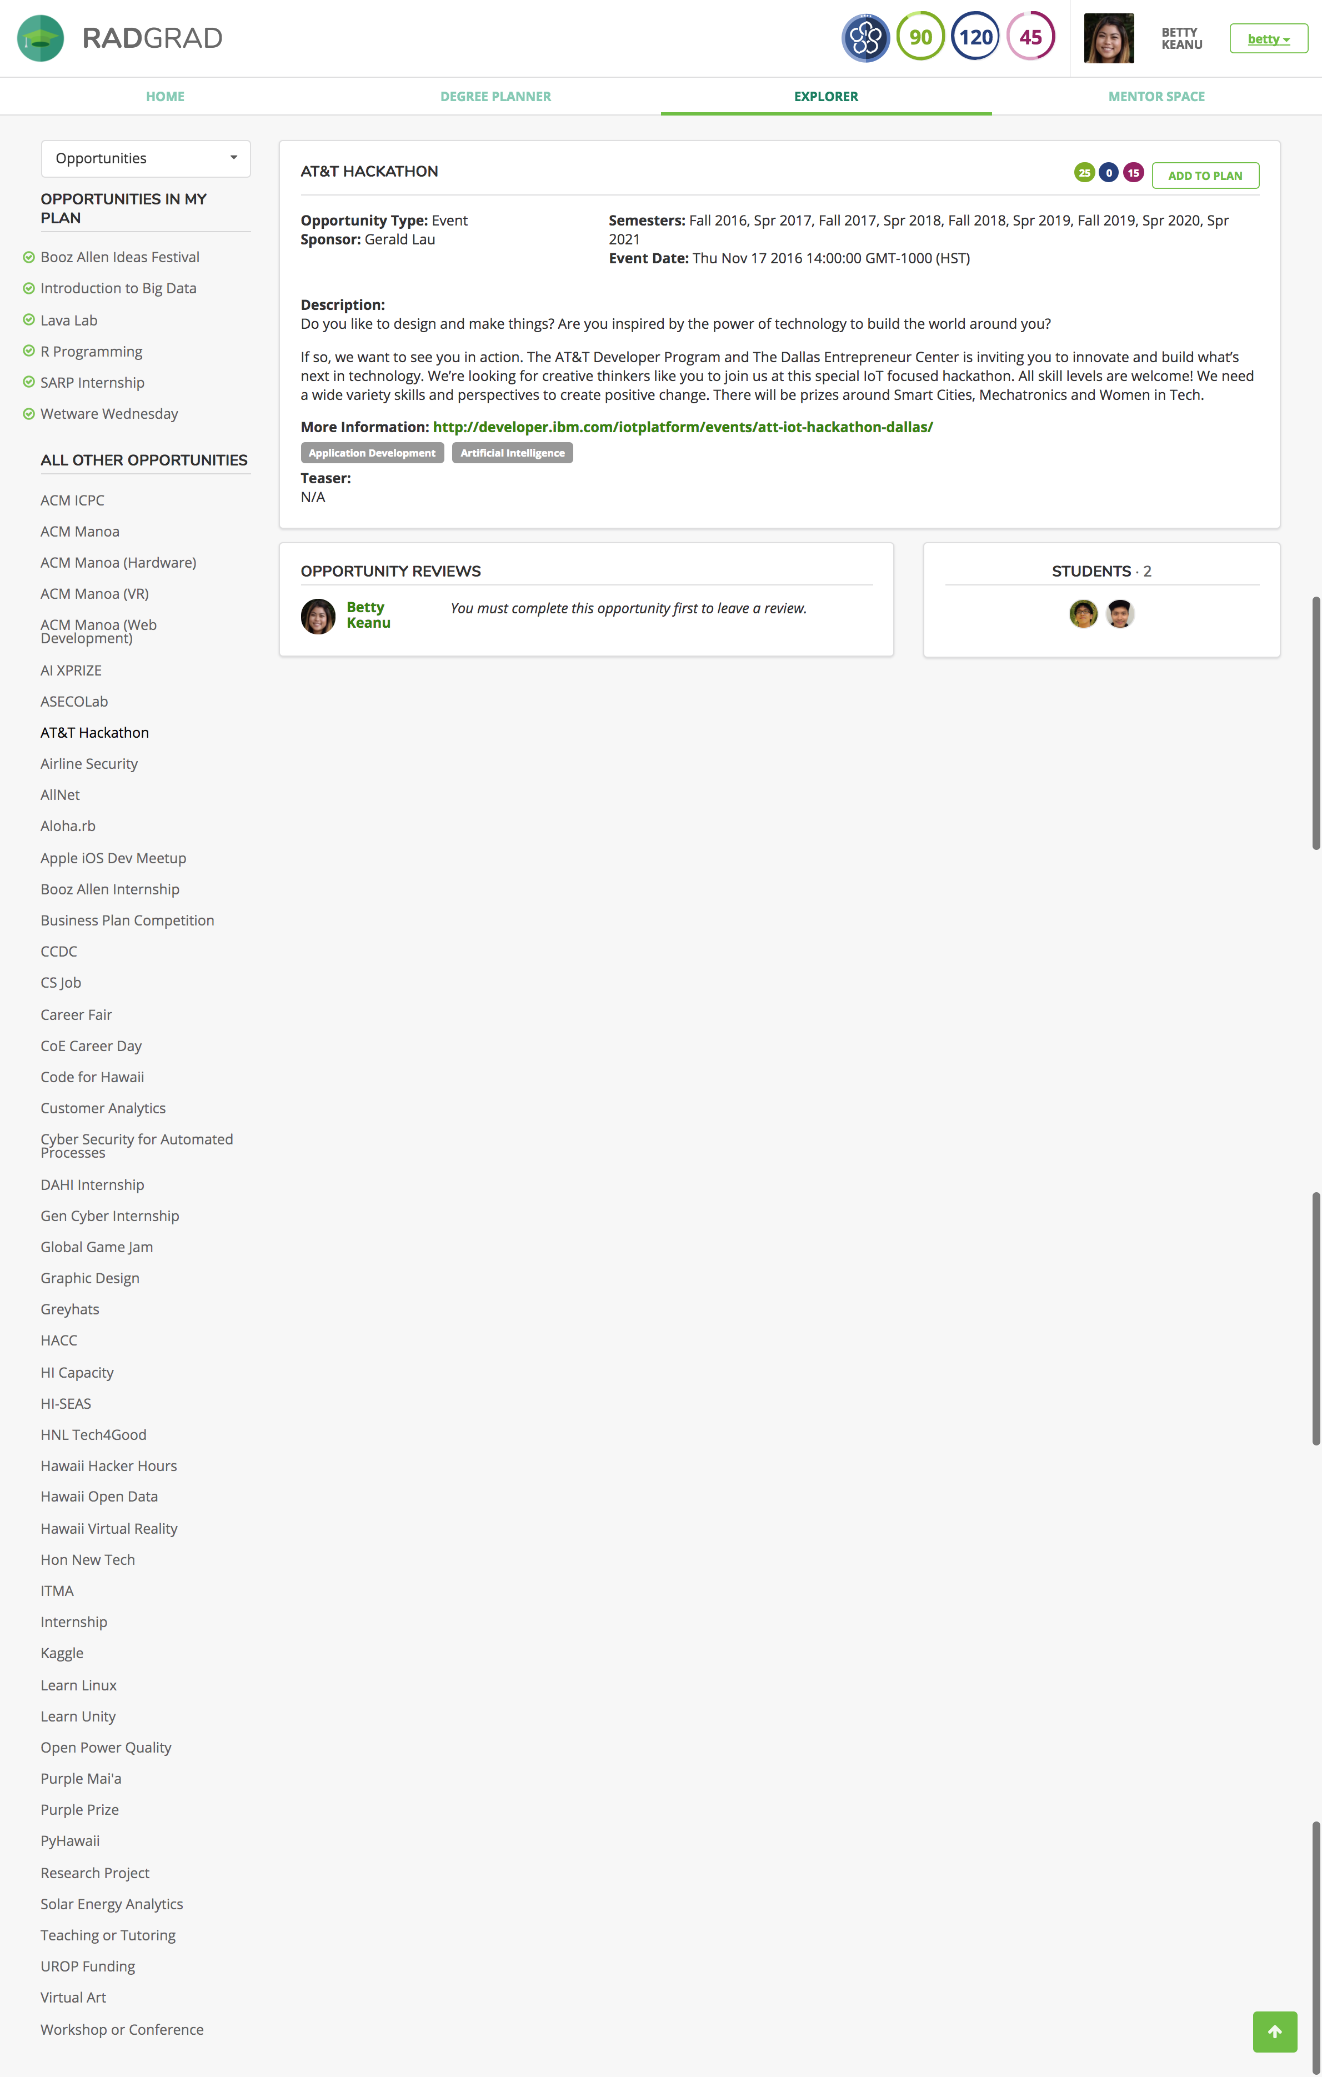
\includegraphics[width=1.0\textwidth]{opportunity-explorer}
\caption{Opportunity explorer page.}
\label{opportunity-explorer}
\end{figure}

The opportunity explorer lists all ICS opportunities on the left side (Figure ~\ref{opportunity-explorer}). These opportunities are arranged by ``Opportunities in my Plan" (all past, present or future opportunities in the user's degree plan) and ``All Other Opportunities" (opportunities not in the user's degree plan). The user can click on an opportunity to view details about that opportunity. These details include the opportunity type, semesters offered, event date, faculty sponsor, a description of the opportunity, related interests, a teaser video, and a list of students with this opportunity in their degree plan. On this page, users can also view opportunity reviews from other students and add or edit their own opportunity review. The user can add or remove this opportunity from their degree plan by clicking on the green button at the top right corner. Unlike courses, users can add an opportunity to their plan as many times as they would like.

\begin{table}[htbp!]
\centering
\begin{tabular}{  |p{4cm}|p{12cm}| } 
\hline
 \multicolumn{2}{|c|}{Potential Areas the Career Goal, Course, Degree, Interest, and Opportunity Explorers Could Improve}\\
  \hline
 \textbf{TechHui Complaints} & \textbf{Reasoning} \\ 
  \hline
ICS department should offer a wider variety of classes & RadGrad explorers allow students to understand their interests, and find various ways to learn about them. Even if ICS does not offer a course in a specific area, students can use the explorer to find other ways to learn (i.e. online courses, interest groups, projects with a professor). \\
\hline
ICS department should offer more focused areas of study & RadGrad explorers allow students to understand their interests, and find various ways to learn about them. Even if ICS does not offer a focus in a specific area, students can use the explorer to create their own personalized degree plan (i.e. adding relevant courses and opportunities, and networking with professors in the area). \\
\hline
ICS classes are too time consuming and take up more time than anticipated & The RadGrad course explorer can help students to gather more information about courses before they take them, including reviews from other students. This type of information can help students to make better informed decisions when creating their degree plan, and they can plan their courses in a way that fits their individual time constraints.\\
\hline
 \textbf{Survey Questions} & \textbf{Reasoning} \\ 
  \hline
  How many extracurriculars have you participated in? & The RadGrad explorers can help students easily find opportunities of interest to add to their schedules.\\
  \hline
  How well prepared do you feel to find a job after graduation? & The RadGrad explorers encourage students to learn more about computer science topics, careers, and opportunities, which can help students get a better idea of, and become better prepared for what they want to do after graduation.\\
  \hline
\end{tabular}
 \caption{Potential Areas the Career Goal, Course, Degree, Interest, and Opportunity Explorers Could Improve}
\end{table}

\subsubsection{Teasers}

\begin{figure}[htbp!]
\centering
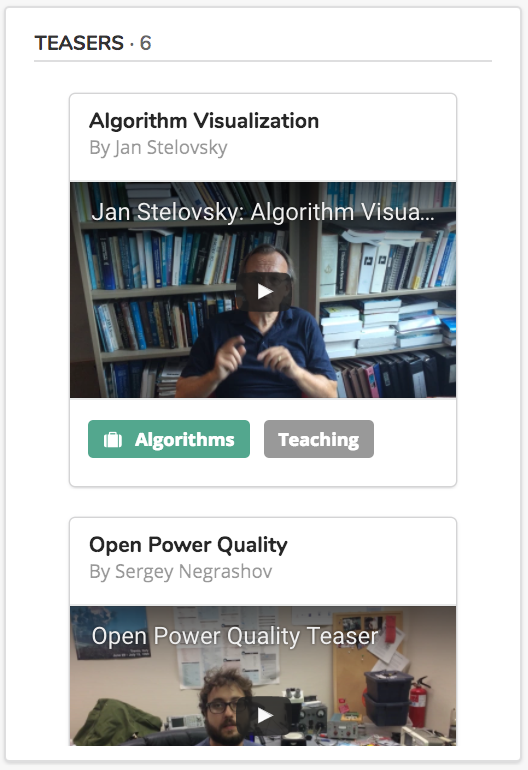
\includegraphics[width=0.5\textwidth]{teaser-widget}
\caption{Close up of teasers on student home page.}
\label{teasers}
\end{figure}
Teasers are short (around 30 seconds) YouTube videos created by members of RadGrad to advertise their opportunity to the rest of RadGrad (Figure ~\ref{teasers}, Figure ~\ref{student-home-page}). Faculty members can create a teaser to help give students an idea of what their current research is about, and students can create a teaser to help give students an idea of what their club or event does and why other students should participate. These teasers supplement the textual opportunity descriptions in the explorer, and appear on the student's home page based off matching interests. Teasers were added on the student home page to serve as eye catching advertisements for opportunities, specifically targeted towards the user.

\begin{table}[htbp!]
\centering
\begin{tabular}{  |p{4cm}|p{12cm}| } 
\hline
 \multicolumn{2}{|c|}{Potential Areas Teasers Could Improve}\\
\hline
 \textbf{Survey Questions} & \textbf{Reasoning} \\ 
  \hline
  How many extracurriculars have you participated in? & Teasers encourage students to add  opportunities of interest to their schedules.\\
  \hline
  How well prepared do you feel to find a job after graduation? & Teasers reinforce the importance of opportunities in students' degree plans.  If teasers successfully encourage students to participate in more opportunities, this can make students more confident and competitive when finding jobs.\\
  \hline
\end{tabular}
 \caption{Potential Areas Teasers Could Improve}
\end{table}

\subsection{Social Network}

The social network components appear on the student home page (Figure \ref{student-home-page}), explorer pages, mentorspace page (Figure \ref{mentorspace}), and several other pages listed below. In the following section, I will describe the social network components in further detail. 

\subsubsection{User Explorer}

\begin{figure}[htbp!]
\centering
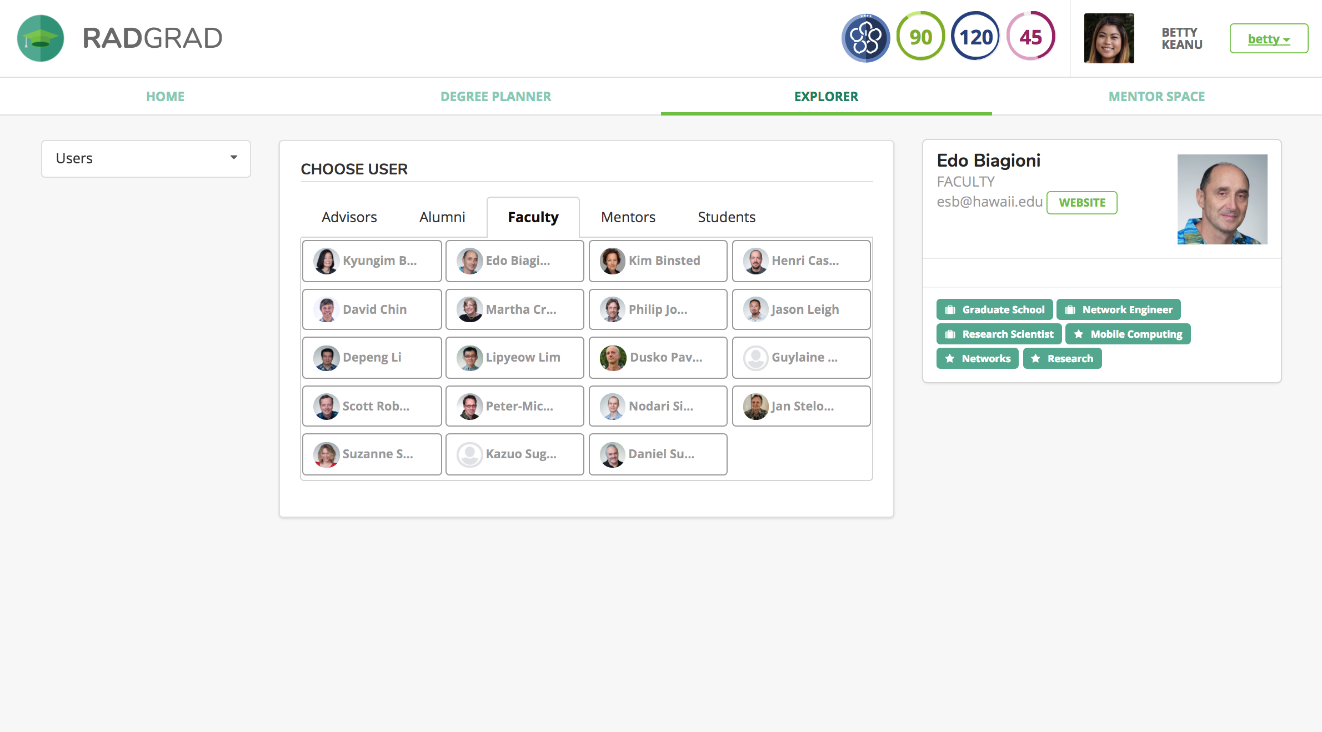
\includegraphics[width=1.0\textwidth]{user-explorer-faculty}
\caption{User explorer page.}
\label{user-explorer-faculty}
\end{figure}

The user explorer lists all RadGrad users with their first name, last name, and avatar (Figure ~\ref{user-explorer-faculty}). Users are arranged in tabs by user type (Advisor, Alumni, Faculty, Mentor, Student) and then listed alphabetically by last name. The current user can click on a user to view details about that user. For student users, these details include desired degree, email, level, taken and planned courses, and completed and planned opportunities. For faculty users, these details include their email, a link to their website, and interests. For mentor users, these details include their email, their MentorSpace answers, and their interests. For advisor users, these details include their email and their interests. Students can use this explorer to learn more about other members of the RadGrad community, and figure out who might be beneficial to talk to (i.e. a higher level student with matching interests and interesting completed opportunities, or a faculty member with matching interests, or a mentor working at the student's dream company). The User explorer was created to encourage more and better social interactions among all members of the RadGrad community.

\begin{table}[htbp!]
\centering
\begin{tabular}{  |p{4cm}|p{12cm}| } 
\hline
 \multicolumn{2}{|c|}{Potential Areas the User Explorer Could Improve}\\
  \hline
 \textbf{TechHui Complaints} & \textbf{Reasoning} \\ 
  \hline
  ICS department should have a better sense of community & RadGrad user explorer can help students learn more about all members of the ICS community, and could potentially facilitate off-RadGrad relationships.\\
  \hline
    ICS courses should involve more group work & RadGrad user explorer can help students easily find and reach out to other students who are in their class or share interests with them.\\
  \hline
  ICS department should encourage more interaction among students & RadGrad user explorer can help students learn more about each other and could help them to interact more both on and offline..\\
  \hline
 \textbf{Survey Questions} & \textbf{Reasoning} \\ 
  \hline
    Do you feel like you get enough support from others in the ICS department? & RadGrad user explorer can help students easily meet people with similar interests and degree plans, and get more support from all members of the community. \\
  \hline
\end{tabular}
 \caption{Potential Areas the User Explorer Could Improve}
\end{table}

\subsubsection{Feed}

\begin{figure}[htbp!]
\centering
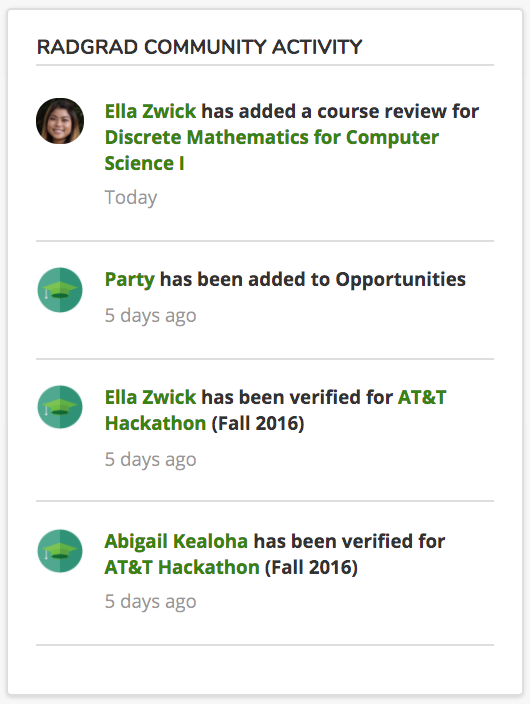
\includegraphics[width=0.5\textwidth]{feed}
\caption{Close up of feed on student home page.}
\label{feed}
\end{figure}
Another way RadGrad reminds users that they are not alone in using the system is by providing a feed on the student home page (Figure ~\ref{feed}, Figure ~\ref{student-home-page}). The feed is one of the first things that a user sees when they log in. Through this feed, users can see events occurring throughout RadGrad such as a new user joining RadGrad, a new course or opportunity is added on RadGrad, a user is verified for an opportunity, or a user has written a new course or opportunity review. The feed provides a single place for students to go to when they want to see what has changed since they have last logged in, and it constantly keeps students updated with the latest changes to the system. Since the feed also allows students to see what other students have been doing, they may be able to get a quick sense of what opportunities are popular among their classmates.

\begin{table}[htbp!]
\centering
\begin{tabular}{  |p{4cm}|p{12cm}| } 
\hline
 \multicolumn{2}{|c|}{Potential Areas the Feed Could Improve}\\
  \hline
 \textbf{TechHui Complaints} & \textbf{Reasoning} \\ 
  \hline
ICS department should have a better sense of community & The RadGrad feed help students to feel like they are part of a larger community and keep up with the latest ICS related events. \\
\hline
\end{tabular}
 \caption{Potential Areas the Feed Could Improve}
\end{table}

\subsubsection{Mentorspace}

\begin{figure}[htbp!]
\centering
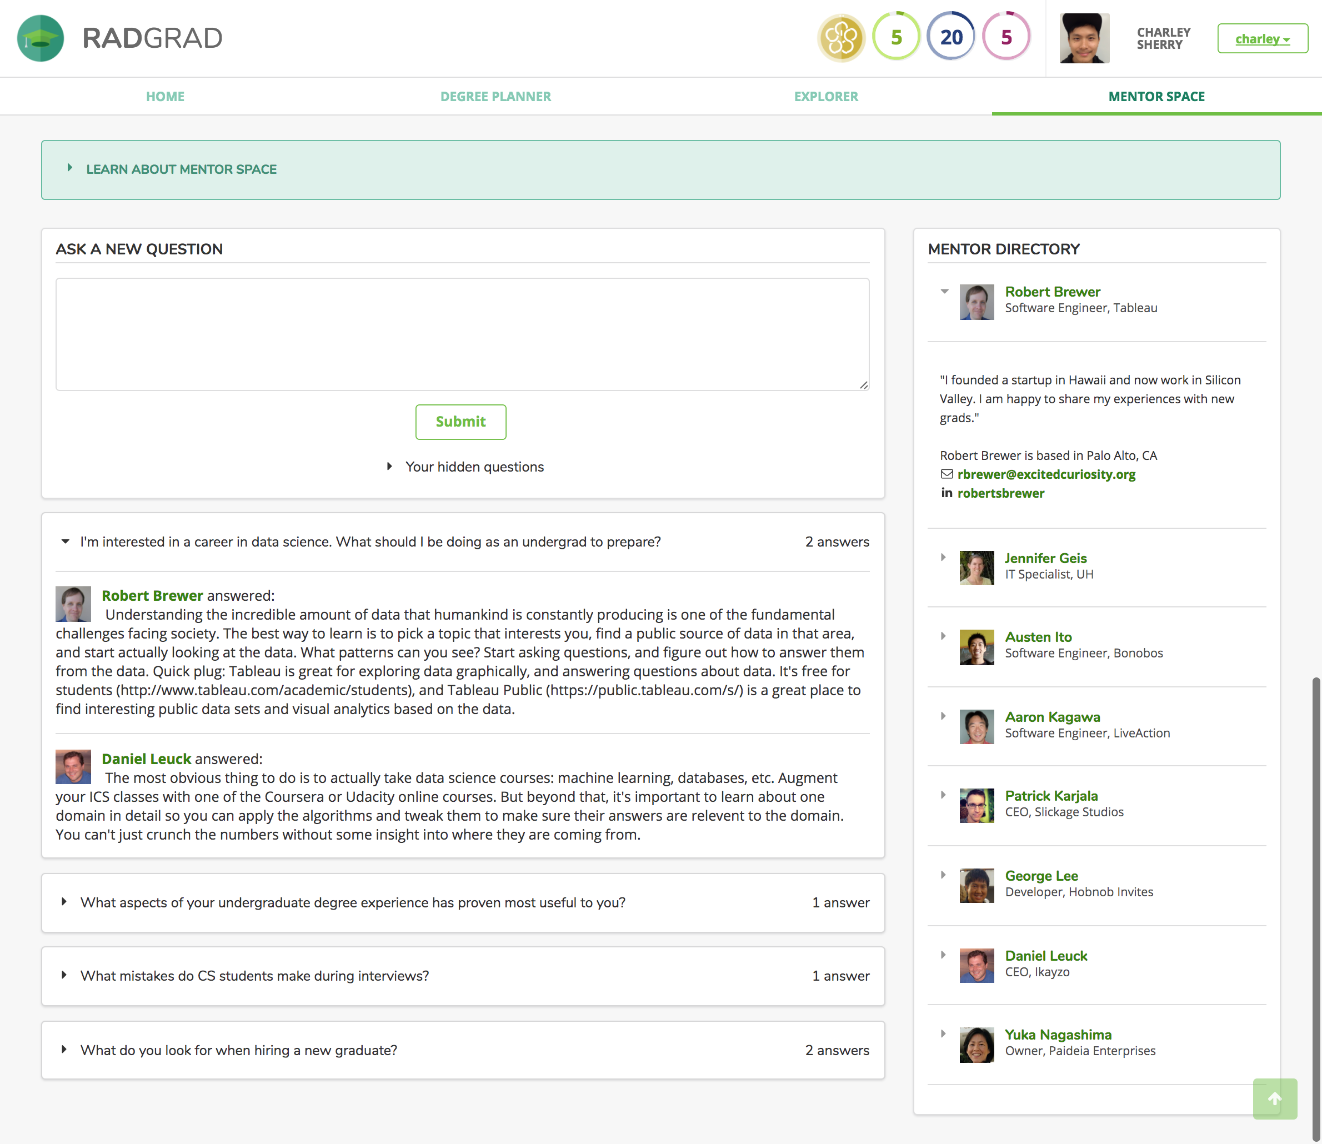
\includegraphics[width=1.0\textwidth]{mentor-space}
\caption{MentorSpace page.}
\label{mentorspace}
\end{figure}
Mentors and students can interact with each other on the MentorSpace page (Figure ~\ref{mentorspace}). MentorSpace was created to encourage more academic and professional interactions between students and alumni. The mentors are listed in the Mentor Directory on the right side of the page. Students can explore who the mentors are by expanding their profile and viewing information about their current company, current location, current job title, email address, LinkedIn, and a description about what inspired them to become a RadGrad mentor. On the left side of the page, students can submit new questions that they have for a mentor. Once the question has gone through moderation (by  Administrators), it will be posted on the MentorSpace for everyone to see. If a question is rejected, it can be edited and resubmitted as many times as desired. A question may be rejected if it contains profanity, is unclear, or is unrelated to ICS. Once a question is posted, mentors can leave an answer for the rest of the community to see. If a student has a specific question for a specific mentor, they can instead contact the mentor through the provided email rather than posting on MentorSpace, which is reserved for questions that can benefit the general ICS student community. 

\begin{table}[htbp!]
\centering
\begin{tabular}{  |p{4cm}|p{12cm}| } 
\hline
 \multicolumn{2}{|c|}{Potential Areas MentorSpace Could Improve}\\
  \hline
 \textbf{TechHui Complaints} & \textbf{Reasoning} \\ 
  \hline
  ICS department should have a better sense of community & RadGrad MentorSpace brings students and mentors together in one place and feel more connected.\\
  \hline
 \textbf{Survey Questions} & \textbf{Reasoning} \\ 
  \hline
  Do you feel like you get enough support from others in the department? & RadGrad MentorSpace can help students get the support they need through questions and answers with mentors who have been in their position before. \\
  \hline
    To what extent have ICS alumni influenced your development in the ICS program? & RadGrad MentorSpace can help students get influenced by alumni both academically and professionally. \\
  \hline
\end{tabular}
 \caption{Potential Areas MentorSpace Could Improve}
\end{table}

\subsubsection{Advisor Log}

\begin{figure}[htbp!]
\centering
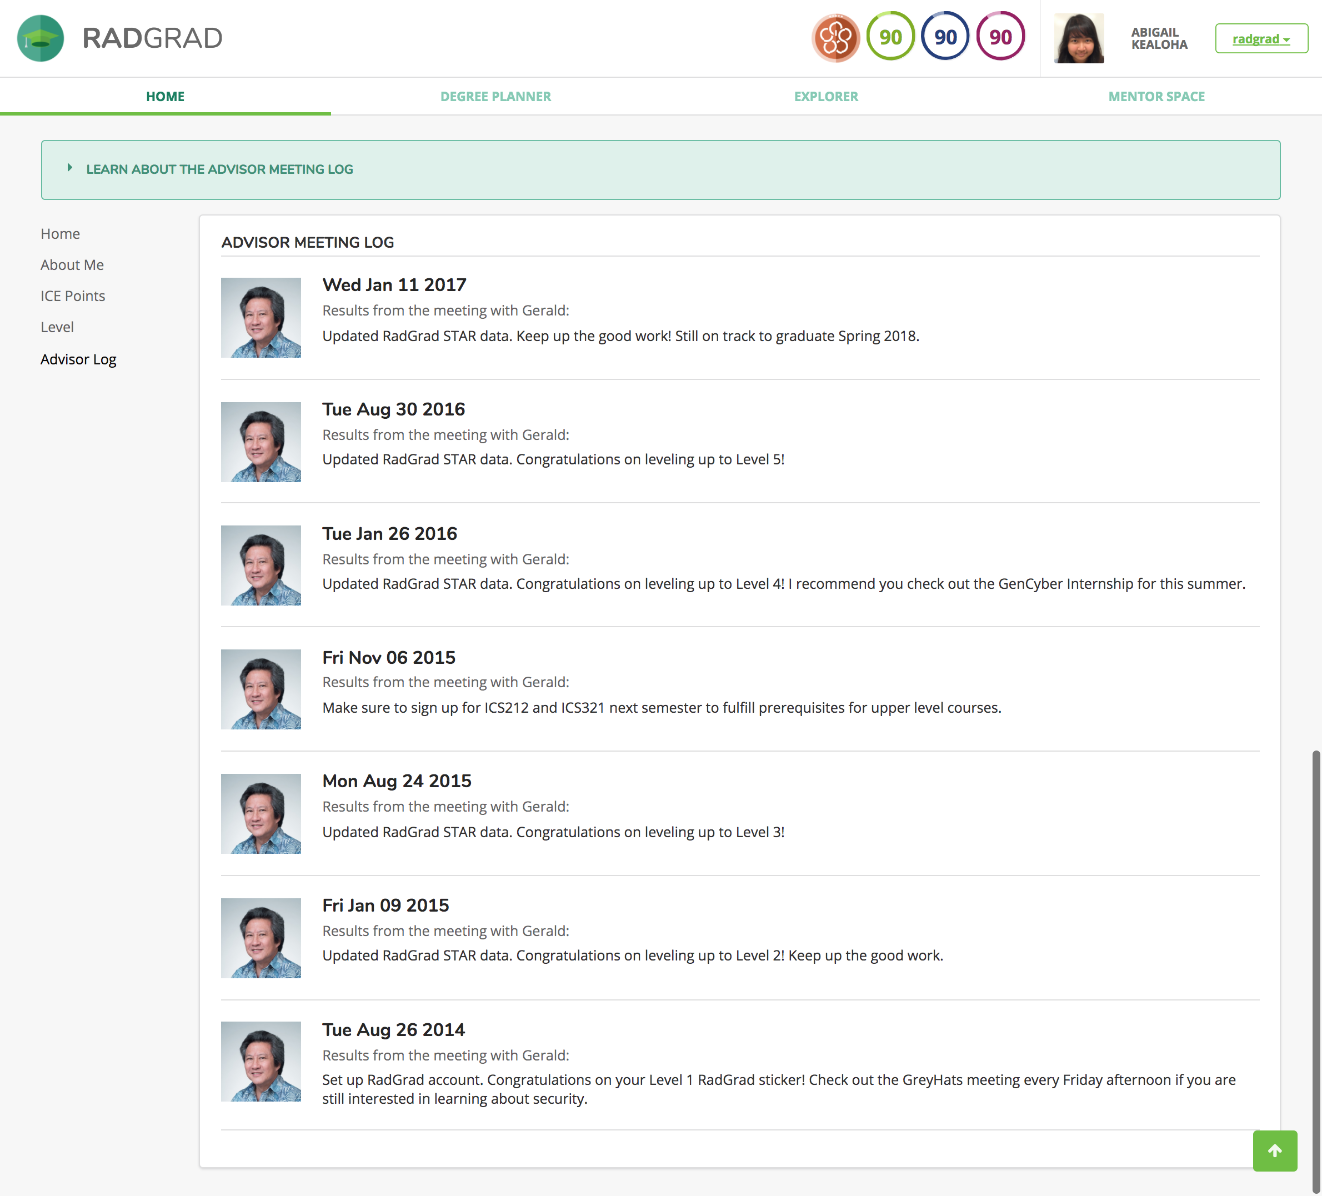
\includegraphics[width=1.0\textwidth]{advisor-log}
\caption{Student advisor log page.}
\label{advisor-log}
\end{figure}
Advisors and students can interact with each other on the Advisor Log page (Figure ~\ref{advisor-log}). Advisor logs were created to help encourage and augment the interactions between students and advisors. When an advisor holds a meeting with a student, he can leave notes from the meeting on the student's Advisor Log. Each log includes a date, the name and avatar of the advisor, and the meeting notes. Advisors can use the log to keep track of their interactions with each student, and students can refer back to the log whenever they can't remember details about what their advisor had said. 

\begin{table}[htbp!]
\centering
\begin{tabular}{  |p{4cm}|p{12cm}| } 
\hline
 \multicolumn{2}{|c|}{Potential Areas the Advisor Log Could Improve}\\
  \hline
 \textbf{TechHui Complaints} & \textbf{Reasoning} \\ 
  \hline
  ICS department should have a better sense of community & RadGrad MentorSpace brings students and advisors together in one place and helps them communicate better and feel more connected.\\
  \hline
 \textbf{Survey Questions} & \textbf{Reasoning} \\ 
  \hline
  Do you feel like you get enough support from others in the department? & RadGrad advisor logs can help students to get more out of their advisors, and can hopefully improve the quality of advisor support and interaction.\\
  \hline
\end{tabular}
 \caption{Potential Areas the Advisor Log Could Improve}
\end{table}

\subsubsection{Reviews}

\begin{figure}[htbp!]
\centering
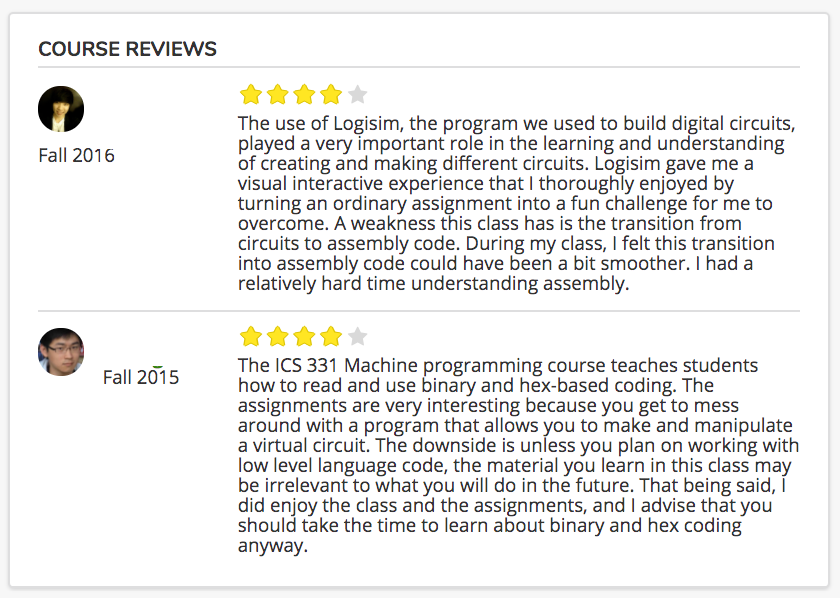
\includegraphics[width=0.5\textwidth]{reviews}
\caption{Close up of reviews on the course explorer page.}
\label{reviews}
\end{figure}
Students can post two different types of reviews: course reviews and opportunity reviews (Figure ~\ref{reviews}). Students can leave reviews for a specific course or opportunity on the course or opportunity explorer page. Students can leave a 1-5 rating and reasons behind their rating. Students can edit or delete their review at any time. Any new or edited reviews immediately appear on the explorer page, but when they go through moderation, they may be removed if they do not abide by the guidelines. Reviews cannot be anonymous, which forces students to take full responsibility for the content of their post. This, along with the fact that all users on RadGrad can view reviews, allows for full transparency between professors and students. Students can view other students reviews to get additional, first hand and anecdotal information about a course or opportunity before they decide to add it to their plan. Faculty and advisors can view reviews to gather feedback about how to improve the ICS program. Reviews encourage more open communication between students and the rest of the RadGrad community and encourages professors to improve, rather than encouraging other students to avoid a certain course, like on Rate My Professors. 

\begin{table}[htbp!]
\centering
\begin{tabular}{  |p{4cm}|p{12cm}| } 
\hline
 \multicolumn{2}{|c|}{Potential Areas Reviews Could Improve}\\
  \hline
 \textbf{TechHui Complaints} & \textbf{Reasoning} \\ 
  \hline
  ICS department should have a better sense of community & Non-anonymous RadGrad reviews help facilitate more open communication between students and the rest of the community.\\
  \hline
    Some ICS professors need to improve their teaching & RadGrad reviews help professors get honest and constructive feedback, which can be used to improve upon their teaching.\\
  \hline
 \textbf{Survey Questions} & \textbf{Reasoning} \\ 
  \hline
    To what extent have ICS peers influenced your development in the ICS program? & RadGrad reviews can help students help others students plan which courses to add to their degree. \\
      \hline
    To what extent have you influenced your ICS peers' development in the ICS program? & RadGrad reviews can help students help others students plan which courses to add to their degree. \\
  \hline
\end{tabular}
 \caption{Potential Areas Reviews Could Improve}
\end{table}

\subsubsection{Avatars}

\begin{figure}[htbp!]
\centering
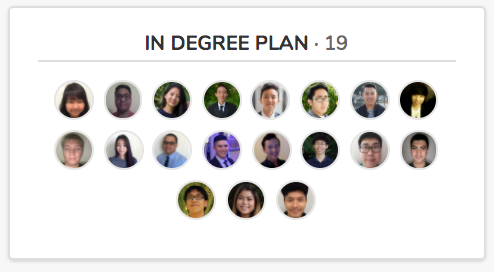
\includegraphics[width=0.5\textwidth]{avatar}
\caption{Example of avatars on the course explorer page.}
\label{course-explorer-avatars}
\end{figure}
RadGrad quietly reminds users that they are not alone in using the system--they are part of a large and diverse network of real people (Figure ~\ref{course-explorer-avatars}). One of the ways RadGrad does this is by incorporating user avatars throughout the site. These avatars appear on the student home page, explorer pages, the user explorer, the student levels page, and the MentorSpace page. These avatars appear to show users related to a certain interest, career goal, course, opportunity, degree, and level. They also are associated with feed items, reviews, and MentorSpace answers. All avatars can be clicked on to navigate to the user's profile in the user explorer.  

\begin{table}[htbp!]
\centering
\begin{tabular}{  |p{4cm}|p{12cm}| } 
\hline
 \multicolumn{2}{|c|}{Potential Areas Avatars Could Improve}\\
  \hline
 \textbf{TechHui Complaints} & \textbf{Reasoning} \\ 
  \hline
ICS department should have a better sense of community & RadGrad avatars help students to feel like they are part of a larger community and help students to get a better idea of the people in the department (i.e. who shares interests with them, who has taken the same courses as them, etc.). \\
\hline
ICS department should encourage more interaction among students & RadGrad avatars help students to find other students that have common interests, and could potentially facilitate relationships off of RadGrad.\\
\hline
\end{tabular}
 \caption{Potential Areas Avatars Could Improve}
\end{table}


\subsection{Gamification}

The gamification components appear on the ICE page (Figure \ref{ice}), the levels page (Figure \ref{levels}), the explorer pages, and several other pages. These components are also constantly present for students to see on any page, on their top menu bar. In the following section, I will describe the social network components in further detail. 
\subsubsection{ICE}
\begin{figure}[htbp!]
\centering
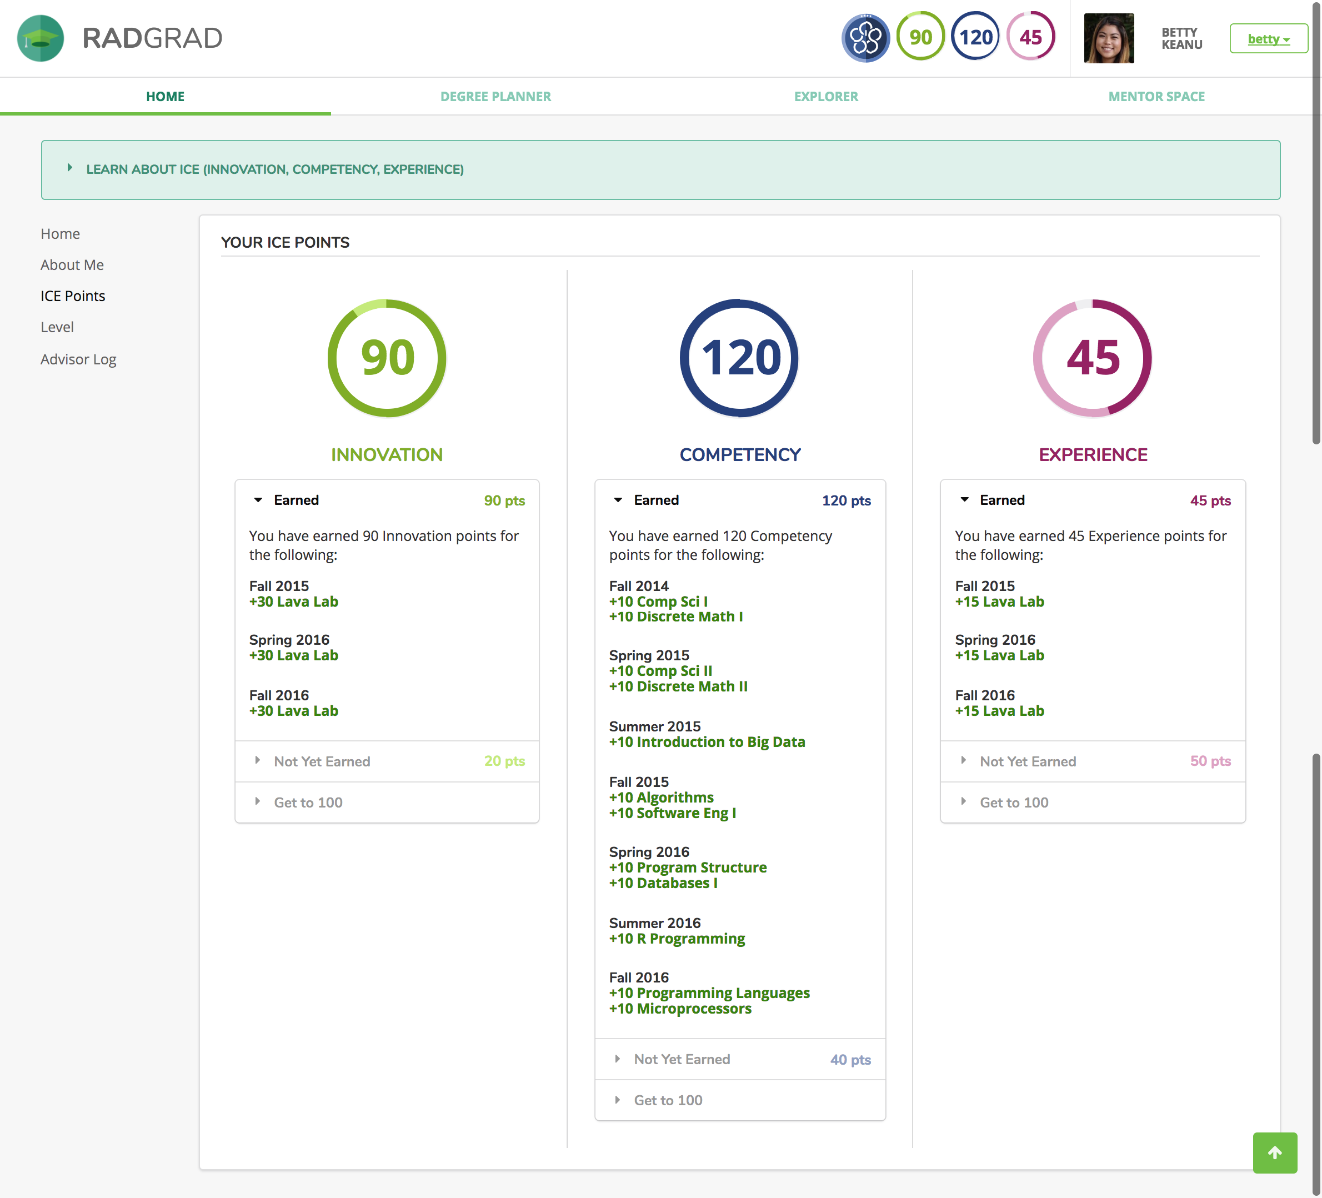
\includegraphics[width=1.0\textwidth]{student-ice}
\caption{ICE page.}
\label{ice}
\end{figure}
ICE is an acronym for Innovation (i.e. a student's involvement in research or other innovative activity), Competency (i.e. a student's grades in ICS courses), and Experience (i.e. a student's involvement in high tech environments through internships or other professional activities). ICE is a measurement of these aspects, calculated using the information provided on the student's profile. Contrasting with traditional requirements that focus solely on GPA, ICE balances the three aspects to emphasize the importance of all three in an ideal ICS experience. The ICE point system can encourage students to become more competitive and give them more incentive to do better.

The student ICE page displays three circular graphs: one each for innovation, competency, and experience (Figure ~\ref{ice}). The number in the center of each graph represents the current amount of points earned for that category. The dark fill in the graph represents the same number. The light fill on the graph represents the amount of planned points. In addition to the student ICE page, these ICE graphs also appear in the top right corner of the menu bar. 

ICE points are also represented for specific courses or opportunities. These ICE points are represented using three filled circles: one each for innovation, competency, and experience. Each circle has a number in the center which represents the amount of points that course or opportunity is worth for that particular ICE category. Students can use these ICE representations to decide which courses or opportunities they should add to their plan, in order to improve their ICE score. These representations appear on the degree planner inspector pane and in the course and opportunity explorer pages. ICE is incorporated in multiple places all over the site to emphasize the importance of well-roundedness, with equal emphasis on innovation, competency, and experience.

\begin{table}[htbp!]
\centering
\begin{tabular}{  |p{4cm}|p{12cm}| } 
\hline
 \multicolumn{2}{|c|}{Potential Areas ICE Could Improve}\\
  \hline
 \textbf{TechHui Complaints} & \textbf{Reasoning} \\ 
  \hline
  ICS department should have a better sense of community & RadGrad ICE can help students to compete and worth with each other to achieve a common goal.\\
  \hline
 \textbf{Survey Questions} & \textbf{Reasoning} \\ 
  \hline
  How well prepared do you feel to find a job after graduation? & RadGrad ICE can help students to gain experience in more areas than just courses. With the "innovation" and "experience" opportunities added to their degree plan, students will have more to offer potential employers than just a decent GPA.\\
  \hline
    How many extracurriculars have you participated in? & RadGrad ICE can help students to participate in more extracurriculars and a wider variety of extracurriculars as they try to reach 100 points in each category. \\
  \hline
\end{tabular}
 \caption{Potential Areas ICE Could Improve}
\end{table}

\subsubsection{Levels}

\begin{figure}[htbp!]
\centering
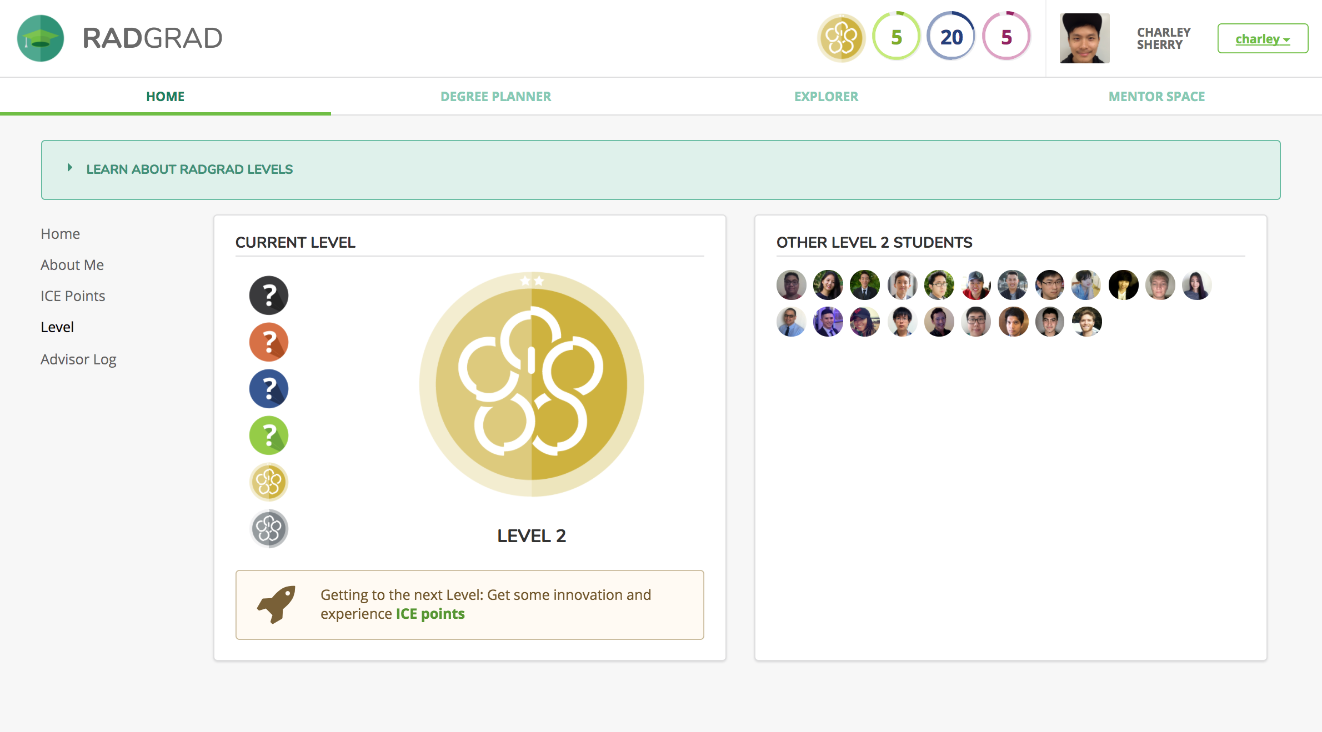
\includegraphics[width=1.0\textwidth]{levels}
\caption{Levels page.}
\label{levels}
\end{figure}

Students can view their current level badge on the student level page (Figure ~\ref{levels}). This page also includes leveling up hints and a list of other students who are at the same level (listed with avatars). This levels page was created to help students to feel a sense of progression throughout their program, and to help them to get to know their peers at the same level.

Levels also persist physically off of RadGrad in the form of stickers. These stickers can be obtained from an advisor or a RadGrad administrator, and a student will receive a new sticker each time they achieve a new level. Students are encouraged to display these stickers on their laptop, as a subtle way to communicate their current standing to their classmates. Using these stickers, students can more easily identify students who are at the same level as them to mingle with, identify students at a higher level than them to get advice from, and identify students at a lower level who could use some peer mentoring. These stickers can also be used to identify current or former ICS students while off campus. In this way, these physical manifestations of RadGrad help to create a sense of ICS community offline as well. 

\begin{table}[htbp!]
\centering
\begin{tabular}{  |p{4cm}|p{12cm}| } 
\hline
 \multicolumn{2}{|c|}{Potential Areas Levels Could Improve}\\
  \hline
 \textbf{TechHui Complaints} & \textbf{Reasoning} \\ 
  \hline
  ICS department should have a better sense of community & RadGrad levels can help students find other students at the same level as them, and also find students who are more advanced and less advanced than them. In this way, students will get a better understanding of those around them.\\
    \hline
  ICS department should encourage more interaction among students & RadGrad levels can facilitate higher level students helping lower level students, and encourage more competition and interaction overall. \\
  \hline
 \textbf{Survey Questions} & \textbf{Reasoning} \\ 
  \hline
   To what extent have ICS peers influenced your development in the ICS program?? & RadGrad levels can help students view other students' level achievements as personal goals, and the levels can also help students choose who they interact with in certain situations (i.e. who to help, or who to go to for help).\\
  \hline
\end{tabular}
 \caption{Potential Areas Levels Could Improve}
\end{table}



\section{Testing}
\subsection{Interactive Testing}

RadGrad uses interactive server-side testing with Mocha test runner and Chai Expect Assertions during code production in order to maintain correctness. Each collection class from the data model has tests in a corresponding testing file. These tests include checking if a new collection entity can be defined, if a collection entity can be removed, if a collection entity can be dumped from the database, and if a collection entity can be restored from a dump file to the database. If the collection class includes additional functions specific to that collection, the test file includes tests for those functions as well.

\subsection{Personas}

In order to ensure that a wide variety of students will be able to use RadGrad effectively, we created five personas, where each persona is represented with a student user account on RadGrad. Each persona represents a student at a different part of the degree program. Below are brief descriptions of each persona. 

\begin{enumerate}
  \item Ella Zwick: Ella is a Freshman who has just declared her BA ICS major. She has not taken any ICS courses yet, and she does not have a RadGrad degree plan yet either. She is at Level 1. Her career goal is to be a web developer, and her interests are in civic engagement and web development. 
  \item Charley Sherry: Charley is a Freshman who is in his second semester of the BS CS curriculum. He is currently enrolled in ICS211 and ICS241. He is at Level 2. His career goal is to be a data scientist, and his interest is in bioinformatics.  He has at least 12 competency points for completing ICS111 and ICS141 during the previous semester. 
  \item Betty Keanu: Betty is a Junior who has completed the BS CS core curriculum (ICS111, ICS141, ICS211, ICS241, ICS311, ICS314) and is currently taking 300+ courses to fulfill the rest of her degree plan. She is at Level 4. Her career goals are graduate school and data scientist, and her interests are big data, visualization, and research. She has completed a few opportunities, and has at least 30 innovation points, at least 36 competency points, and at least 30 experience points. 
  \item Abigail Kealoha: Abigail is a Junior who is two semesters away from graduating with her BS in CS. She is Level 5. Her career goal is to be a web developer, and her interests are security and software engineering. She has completed several opportunities, and has at least 80 innovation points, at least 80 competency points, and at least 80 experience points. Abigail has also contributed one course review on RadGrad. 
  \item Alfred Persona: Alfred is a Senior in his last semester of the BS CS curriculum. He is at Level 6. His career goal is a software developer and his interests are in game design, hardware, and virtual reality. He has completed many opportunities, and has at least 100 points for each of the ICE categories. Alfred also contributed 6 course reviews on RadGrad.
 
\end{enumerate} 

The RadGrad team used these personas to test different scenarios while building the interface. For instance, these personas were useful when testing different how types of degree plans appear in the degree planner. These personas were also useful when testing how the different components on the student home page would appear for different types of students (i.e. students with few versus many interests, students who have completed many versus few courses and opportunities, etc.) We also used these personas when we calculated specific gamification aspects, in order to make sure the games were challenging enough, but not unreasonable. 
 
\subsection{Beta Testing}

In Spring 2017, after completion of the major Student, Advisor, and Administrator components and pages, we held RadGrad beta tests, which invited selected students and an advisor to view and use the system for the first time. The main goals of these tests were to identify user problems, identify common aspects users like, assess if parts of the user interface are more intuitive or more difficult to use, if there are missing features that should be implemented, if certain features could be improved, and to get a feel of whether users feel that the would use RadGrad and that it would improve their engagement in the ICS degree program. We hoped this data would help us decide if the system so far is going in a promising direction.

\subsubsection{Student Beta Testing}

Student subjects were solicited over email, and were selected in a way that provided us with a wide range of student levels. Each student was given \$20 as compensation for 30 minutes of their time. Prior to the testing session, each subject provided their name and UH account, completed ICS courses, completed opportunities, interests, and career goals. Using this information, the student's RadGrad account was set up prior to the session. Each session involved one student and two RadGrad developers (an evaluator to lead the session, and an observer). At the start of the session, the evaulator briefly went over the basic ideas of the system and the different parts that they can interact with. During the second part of the session, the student was allowed to peruse the system and explore or comment on anything they found particularly interesting. During this time, students were given some basic tasks to accomplish (e.g. to find some courses of interest and add them to their degree plan), and were also given time for open exploration. During the third part of the session, the evaluator asked the student to describe what they liked about the system, what they disliked about the system, and whether or not they think they would use this system if it were available to them. The goal of the beta testing was to discover any basic functionality problems, and to get feedback from real students on whether they would find certain features appealing or not. See Table ~\ref{table:student-beta-test-results} for the student beta testing feedback.

\begin{table}[htbp!]
\centering
\begin{tabular}{ |p{8cm}|p{8cm}|}
 \hline
\textbf{Positive Feedback} & \textbf{Problems with System} \\
 \hline
 Recommended opportunities are useful because otherwise students are only notified by Gerald's emails  & ICE points display was confusing \\
 \hline
 Reduces the amount of work currently needed for students who try to find ways to succeed beyond the classroom. &List of opportunities was hard to view because it was partially off the screen\\
 \hline
 Degree planner helpful for visualizing pathway &Annoying to have to scroll to see all possible review ratings\\
  \hline
Likes the levels and ICE gamification &Confusing to find some things without some kind of tutorial \\
 \hline
Level stickers can help students see who they might want to talk to &Performance issue with page loading times \\
 \hline
RadGrad and ICE are good at stressing the importance of activities outside of courses &Wish there were notifications for when new opportunities come up\\
 \hline
RadGrad provides extra details about courses and opportunities that were previously unknown to the student &Recommended Courses and Recommended Opportunity widgets on the student home page have non-intuitive scrolling behavior\\
 \hline
RadGrad helps degree plan to feel less ``random" &Wish there were notifications for when new opportunities come up\\
 \hline
Likes how RadGrad helps students understand the benefits of internships, which they learned too late would be helpful &Students should be allowed to opt out of showing their current and future courses and opportunities\\
 \hline
RadGrad is a good way to keep track of a degree plan, which a student previously wrote on a paper and misplaced it & Wish there were notifications for when new opportunities come up \\
 \hline
 STAR does not work adequately for many students, and RadGrad could be a good supplement for that & Wish there was less unnecessary clicking while altering the degree planner\\
 \hline
Student easily navigated degree planner UI with only some guidance &Wish there were support for specific focus areas\\
 \hline
Mentorspace could help students to get an idea of what they can actually do with their degree after graduation &Would like to know ahead of time when certain courses are being offered\\
 \hline
The fact that RadGrad helps you plan even if you have no idea what you want to do, whereas with STAR, you have to know what you want to do beforehand & Manual edits to one student's generated plan caused empty extraneous years in the degree planner\\
 \hline
Rating courses seems helpful in planning & One student's STAR data included a long gap between years, which wasn't handled well in the degree planner without manual intervention\\
 \hline
Liked how degree plan could be generated rather than manual &\\
 \hline
Liked the idea of an individual ICS online space &\\
 \hline
\end{tabular}
\caption{Student beta test results}
\label{table:student-beta-test-results}
\end{table}

\subsubsection{Advisor Beta Test}

It was easier to solicit an advisor for the beta test, since Gerald Lau is currently the only ICS advisor. During his session, the evaluator briefly went over the system from the point of view of both students and the advisor. While Gerald did not actually get to interact with the system himself, he was able to see how it would be used, and he was able to give feedback about his perceived usefulness of the system. Gerald's response was positive overall, and he seemed interested in integrating it into future advising.